% Two sided means the left and right margins are different sizes and they alternate every page. 
% If your document is printed to be book or spiral bound this allows for a thick spine to not 
% eat into the space for your page content. 
\documentclass[11pt, a4paper, twoside, openright]{custard}

% All imports, packages, and configuration in here. 
% Your document should be about content so we abstract away the styling rules and tools we are using. 
%% Here you can specify new commands and environments that you intend
%% to use. Using commands can make your document easier to write, read
%% and be more consistent.

\usepackage[linesnumbered,ruled]{algorithm2e}
\DeclareMathOperator*{\argmin}{arg\,min}

\usepackage{appendix}
\usepackage{textcomp}
\usepackage{setspace}
%\usepackage[document]{ragged2e}
\usepackage{verbatim}
\usepackage{multirow}
\usepackage{multicol}
\usepackage{booktabs}
\usepackage{enumitem}
\sloppy
\usepackage{graphicx}
\usepackage{threeparttable}
\usepackage{epsfig}
\usepackage{epstopdf}
\usepackage{float}
\usepackage{enumitem}
\usepackage{cite}
\usepackage[export]{adjustbox}
\usepackage{algorithmic}
\usepackage[nohyperlinks,printonlyused]{acronym}
\usepackage{amsmath}
\usepackage{amsfonts}
\usepackage{array}
\usepackage{tabularx}
\usepackage{longtable}
\usepackage{times}
\usepackage{amssymb}
\usepackage{hhline}
\usepackage{color}
\usepackage{soul}
\usepackage{colortbl}
\definecolor{Gray}{gray}{0.85}
\usepackage{rotating}
\usepackage{fix2col}
\usepackage{pdflscape}
\usepackage{pdfpages}
\usepackage{stmaryrd}
\usepackage[export]{adjustbox}
\usepackage{bbm}
\usepackage{relsize}
\usepackage{xfrac}
\usepackage{bibentry}
\usepackage[super]{nth}
\usepackage[xcolor,leftbars]{changebar}
\usepackage{pdfpages}
%\usepackage{pythontex}

%\usepackage{refcheck}

%watermarking
\usepackage[english]{babel}
\usepackage{tikz}

%% Uncomment the following line for hyper links - not recommended for printing
\usepackage[colorlinks, linkcolor=, anchorcolor=, citecolor=, filecolor=, menucolor=, runcolor=, urlcolor=]{hyperref}

\setcounter{tocdepth}{1}
%\setcounter{minitocdepth}{3} 
\linespread{1.31}

\newcommand\litem[1]{\item{\bfseries #1:\enspace}}

\interdisplaylinepenalty=2500

\newcolumntype{L}[1]{>{\raggedright\let\newline\\\arraybackslash\hspace{0pt}}m{#1}}
\newcolumntype{C}[1]{>{\centering\let\newline\\\arraybackslash\hspace{0pt}}m{#1}}
\newcolumntype{R}[1]{>{\raggedleft\let\newline\\\arraybackslash\hspace{0pt}}m{#1}}

\renewcommand{\thefootnote}{\fnsymbol{footnote}}
\setlength{\LTpre}{-10pt}\setlength{\LTpost}{-30pt}%
\newcommand{\oiint}{\begin{picture}(0,0)(-10,-2)\put(0,0){\oval(12,8)}\end{picture}\iint}
\renewcommand{\mathbf }{\boldsymbol}

\def \eg{e.g.\ } % Allows you to write \eg in LaTeX instead of typing e.g. so that every single one will be formatted the same.
\def \Eg{E.g.\ } % Define some other common variants. If you later want to change one of these definitions, 
\def \ie{i.e.\ } % it will update all the usages throughout the document.
\def \Dr{Dr.\ }
\def \vs{vs. }
\def \etal{\emph{et al.\ }} 
\def \sota{state-of-the-art }
\def \handcrafted{hand-crafted }

\usepackage{listings,lstautogobble}
\usepackage{sourcecodepro}
\pdfmapfile{=SourceCodePro.map}
\lstset{
	xleftmargin=0.5cm,frame=tlbr,framesep=4pt,framerule=0.5pt,
	language=,
	upquote=true,
	columns=fixed,
	tabsize=2,
	extendedchars=true,
	breaklines=true,
	numbers=left,
	numbersep=10pt,
	basicstyle=\ttfamily\scriptsize,
	numberstyle=\tiny,
	stringstyle=\ttfamily,
	captionpos=b,
	showstringspaces=false,
	autogobble=true
}

\usepackage[font=small,skip=10pt]{caption} %,format=hang
%\usepackage[labelformat=simple]{subcaption}
\usepackage[labelformat=simple]{subfig}
%\captionsetup[figure]{format=hang}
%\captionsetup[lstlisting]{format=hang}
\renewcommand{\thesubfigure}{\Alph{subfigure}.}

\renewcommand{\thefootnote}{\arabic{footnote}}

% Use IEEEtran citation style. 
\bibliographystyle{IEEEtran} 

\def\samplefont#1{%
    % set font style and save name
    #1\edef\savedname{\fontname\font}%
    % print small sample
    {\leavevmode\tt\hbox to 1in{\savedname:\hss}}%
    abcxyz ABCXYZ 123\par
}

\begin{document}
	
% The custom data for Swansea University and your degree name.
% The \protect\\ command forces a new line in the title which might be otherwise overriden by the template
	\title{Data Splash! \protect\\An Educational Game about Machine Learning}
	\author{Andrew Gray\protect\\{\normalsize 445348}}
	\awardinginst{Swansea University}
	
% Comment / uncomment your degree type as needed.
	%\degree{Bachelor of Science} 
	\degree{Master of Science}
	%\degree{Doctor of Philosophy}
	
% Institution details and logo
	\department{Department of Computer Science}
	\university{Swansea University}
	\unilogo{graphics/swansea.png}
	\date{September \nth{20}, 2020}
	
% Hard code the date or allow the LaTeX compiler to fill it in whenever you recompile the document.
	
	
% Build the title and declaration pages, and pad the document so the text starts on a right hand book page.
% Page numbering is in roman numerals until the first page of an actual chapter which resets numbers 
% starting from 1 at that point. 
	\frontmatter%
	\maketitle
	\declaration
	\cleardoublepage
	
% Most books and theses have a brief foreword or dedication. 
	\begin{vplace}[0.7]
		\begin{large}
			\begin{center}
				\textit{I would like to dedicate this work to the Hypnotoad.\\All glory to the Hypnotoad.}
			\end{center}
		\end{large}
	\end{vplace}

% Abstract comes before the contents page.	
	\begin{abstract}
		\vspace{-2em}
		\setcounter{page}{1}
		
		In your abstract you should aim to summarize the core contributions of your work in the context of the problem domain. Start by outlining the domain and the problems posed within it. Discuss how the methods you focus on approach the relevant problems. You should end your abstract by concretely stating the tangible outputs and deliverables you have created in order to complete your work on this document, and whether those outputs represent and improvement or alternative approach to existing methods. 
		
		Your abstract should be a couple or so paragraphs long, and roughly approximate the order and flow you then use for structuring the main document. If a viewer has read your abstract then they should already understand at a high level what it is you have created and delivered, and whether it is better than or comparable to existing methods. If your project is driven by a research hypothesis then the reader should know what that is at a high level from this section. Reading on, little should surprise the viewer.
		
		For paper submission of your thesis you should physically sign your name on each of the above declaration statements and date them in black ink. For digital submissions you should sign and date them digitally using a touch or stylus input if available. There are pieces of software that allow you to write directly on PDF documents, or alternatively you can bring a signature into your document as a figure with a transparent or white background. If you do not have a stylus input / tablet like device you should ask your supervisor, as many in the department do their grading / work on digital tablets.
	\end{abstract}
	
% A long form dedication. 
	\begin{Acknowledgements}
		This is an opportunity to acknowledge and thank those who have supported you throughout your studies. Friends and colleagues who you have studied alongside, your families, and your mentors within the department are the usual suspects. 
	\end{Acknowledgements}
	
% Build the table of contents page.
	\tableofcontents*
	 
% Optionally you can make a bank of known acronyms in acronyms.tex that you can call on throughout your document.
	%\input{acronyms} 
	
% For long documents like a Doctoral thesis you should include a list of tables and figures throughout 
% your document. This is uses a shortened version of each table and figures caption and enumerates all 
% of them with their table or figure number. This is automatic, you do not need to modfy it if you do use it.
	\setlength{\columnsep}{10pt}
\newpage
\listoftables
\mtcaddchapter 
\newpage
\listoffigures
\mtcaddchapter  
	
% Reset numeric page numbering from page 1
	\mainmatter%

% Insert the code for each of your chapters
	\chapter{Introduction}
	\label{chap:intro}
	
	This document is intended both as a thesis template and a written tutorial on typesetting a professional looking academic document. The style of the template is designed to mimic an equivalent LaTeX document template that is commonly used for within the Computer Vision and Visual Analytics group here at Swansea. This LaTeX template is itself based on a LaTeX template named Custard. 
	
	\section{Motivations}
		\label{sec:intro_motivation} 
		
		Large documents can become cumbersome to work with and format consistently. Sensibly chosen aesthetic cues are important to help imply structure and can greatly aid the reader in understanding your work. The accompanying LaTeX template uses abstraction to hide the formatting from the author during content preparation, allowing for consistent styling to be applied automatically during document compilation. In this Google Docs theme it is the responsibility of the author to manually adhere to the styling laid out in this template.
	
	\subsection{Objective}
		\label{sec:intro_objective} 
		
		In this document we present a tutorial on thesis creation and typesetting, and discuss topics such as literature surveying and proper citation. 
		
	\section{Overview}  
		\label{sec:intro_overview} 
		
		The remainder of chapter \ref{chap:intro} outlines the document structure and the key contributions of this work is organized as follows. Chapter \ref{chap:resources} reviews techniques for finding and properly citing external resources from the academic literature and online. In chapter \ref{chap:typesetting} we show examples of how to typeset different types of content, such as internal references, figures, code listings, and tables. And lastly in chapter \ref{chap:conclusion} we summarize the main contributions and key points to take away from this template.
	
	\section{Contributions} 
		\label{sec:intro_contribs} 
		
		The main contributions of this work can be seen as follows:
		
		\begin{description}	
		
			\item[$\bullet$ A LaTeX thesis template]\hfill
			
			Modify this document by adding additional TeX files for your top level content chapters. 
			
			\item[$\bullet$ A typesetting guide of useful primitive elements]\hfill
			
			Use the building blocks within this template to typeset each part of your document. Aim to use simple and reusable elements to keep your LaTeX code neat and to make your document consistently styled throughout.
			
			\item[$\bullet$ A review of how to find and cite external resources]\hfill
						
			We review techniques and resources for finding and properly citing resources from the prior academic literature and from online resources.
			
		\end{description}
	\chapter{Background \& Literature Review}
	\label{chap:background_lit_review}
	
	To be able to implement our application, with the desired outcomes, we must first look into several key topics backgrounds. First, we will be looking into educational games, and what makes something an educational game. Then we will be looking into a motivational feature called gamification and how it is used in education and within greater science concepts. As well as the different types of ML models and different ways these models are currently getting taught to potential students.
	
	We wanted to find out what the context of gaming and what gamification is, and how it can be used within education, to take aspects of teaching and learning that can get brought into the 21st Century. To make aspects of education more accessible to students in a manner that they are more accustomed to in their everyday lives. 
	
	\section{Introduction to Educatiuonal Games}
		\label{sec:intro_to_edu_games}
	
	Games that get designed with educational purposes as its intention, or that have incidental or a secondary educational value get categorised as educational games. Although` all types of games can get used within an educational setting. However, only games that get designed to help learners learn about certain subjects, expand concepts, reinforce development, understand a historical event or culture, or assist them in learning a skill as they play can get classed as an educational game. Game types include board, card, and video games. As educators, governments, and parents realise the psychological need and benefits that gaming has on learning, this educational tool has become mainstream \cite{barab2009transformational}. 
	
	Research suggests that there are three main approaches to creating software that stimulates cognitive growth within a gamer. These are building games from scratch that have been created by educators and programmers, integrating commercial off-the-shelf games and finally creating games from scratch, which have been done by the students \cite{van2006digital}. For these to work these approaches requires the teacher to buy into the positive results of using digital games for education. It also requires teachers to have adequate self-efficacy concerning the use of these games and their technology. The students usually have high amounts of self-efficacy in the usage of digital games. In contrast, the lack of confidence teachers have in incorporating digital games usually results in the delivery of less effective educational use of the games. However, Gerber and Price have found that teachers' inexperience with digital games does not prevent them from the desire to incorporate them in-class instruction \cite{gerber2013fighting}.
	
	
	\subsection{Gamification}
	%%% From HCI Report
	Gamification, a term first coined in 2002, is an HCI technique used to add a game layer to traditional non-game like situations. Gamification aims to create extrinsic motivators for a person to be encouraged to do particular actions. Each action, upon completion, will have a little reward which, upon doing so, will release dopamine into the brain. The release of dopamine creates a good feeling within the participant's mind, which in turn encourages them to do it again. These rewards can be in the form of badges, achievements or progress bars, to name a few.
	
	The term gamification first appeared in the context of software design in 2008 \cite{4}, but the term got more widespread recognition within 2010. However, the term "gamification" was first coined by Nick Pelling in 2002 \cite{3e}. His initial aim with gamification was to combine the social and rewarding features of games into the software. Gamification started to gain much attention, so much so that it got described as one of the most promising areas of gaming \cite{5}. Gamification is now known as a powerful tool for engagement, which has, since its initial conception, now becoming a conventional feature within software development \cite{3e}. Researchers consider gamification to be the progression of earlier work that focuses on adopting game-design elements to non-game situations and contexts. Research in the HCI field, in regards to apps that use game-driven components for motivation and also in interface design, suggest that there is a connection between Soviet concepts of socialist competition and the American management trend of "fun at work" \cite{5}.
	
	Jane McGonigal, in 2010, delivered a groundbreaking TED Talk titled, "Gaming Can Make a Better World' \cite{6}. This talk is known as the defining moment in the history of gamification. During the talk, she foresees a game based paradise as she states within her talk "I know two things for sure: that we can make any future we can imagine, and we can play any games we want, so I say: Let the world-changing games begin \cite{6}." Hindsight shows she was correct, as, from 2011, gamification starts to pick up steam.  At a Computer-Human Interaction (CHI) conference, a workshop titled "Gamification: Using Game Design Elements in Non-Gaming Contexts \cite{7}", which in the year of 2011 created the Gamification Research Network (GRN) \cite{11}. Through the following years, gamification continues to grow. Gamification goes viral without people knowing through a game called Pokémon Go where it became one of the most successful applications of gamification ever, with over 800 million downloads. People who would usually turn their nose up at badge collecting were out walking the streets searching for rare Pokémon. Pokémon Go is one of the most successful apps of all time, so much, so it even broke records \cite{3e,8}. It could be said thanks to Pokémon Go, that gamification is now everywhere.  
	
	%%%%%%%
	
	
	\subsection{Gamification in Education}
	%%% Taken from HCI report
	The gamification within a learning setting is a pedagogical approach to motivate students. This approach tried to help students learn by using gaming elements within a learning environment \cite{22}. Gamification within education is very much the same thing, in general, as gamification. However, within education, it has a focus on aiding learning instead. Gamification in learning has two main views. One of the views categories gamification of learning as learning which has game-like characteristics. However, this view believes it is only the case when only when the learning is happening in a non-game setting, like a classroom. This view would involve a range of elements that get presented in a  game layer which attempts to happen alongside the learning in a traditional classroom. The other view has the same views as the view just mentioned, but the other half also include games that get designed to provoke learning within them \cite{22}. 
	
	Gamification, within an educational or a learning situation, has many benefits. While traditionally gamification has been used to improve attendance with incentives by reaching a set score or receiving extra prizes for completing designated tasks within a lesson. It can also aid in cognitive development within youngsters, which can boost levels of engagement and can assist with accessibility within the classroom \cite{24}. Games that get created for improving cognitive development are known as "brain games" \cite{24}. These popular games typically are focused around a series of questions and problems to solve or answer. These games develop the rate the player can sustain information and increase the brain's ability to process knowledge. The levels of the engagement increases when gamification has gets used within a classroom \cite{25}. A study performed by scientists aimed to measure the students' levels of engagement in a classroom where gamification elements are applied \cite{25}. They assigned a point system to multiple daily activities, and every student had a measurement of their observed level of engagement. The finding showed that the game like setting was supporting the learning within the classroom and increased productivity. Therefore, by increasing engagement levels, it also means it helps students be able to access the content of the lesson better. 
	
	Gamification of learning has excellent potential benefits. The gains allow students to have ownership of their education, as well as giving opportunities for the learner to gain a sense of their "own identity" through alternative role-playing selves. The freedom that gets bundled without any negative repercussions allows the students to fail and keep on trying again. The ability to increase fun and joy while learning. The opportunity for tasks to be differentiated. Making the learning visible and providing opportunities to inspire intrinsic motivators for learning. Also, the ability to aiding in motivating students with low levels of motivation \cite{22}. 
	
	Even though gamification can aid teaching students of all needs, a study conducted on students who had autism using video games showed that this training method was powerful in teaching the content that was age-appropriate \cite{26}. However, gamification of learning is not something just for the classroom. It is an excellent tool for learning outside the classroom and allowing education to get conducted without an educational facilitator like a teacher. 
	
	%%% Taken from CSCM10 Report
	\subsection{Gamification in Science}
	\label{sec:game_in_science}
	
	The National Research Council report argued that science is the discipline that should convey those skills required for a twenty-first-century workforce, such as non-routine problem solving, adaptability, complex communication/social skills, self-management, and systems thinking \cite{national2010exploring}. Creating a scientifically literate population requires a strong science education \cite{morris2013gaming}. This statements spawned a focus on how video games have the potential to be exploited for gain in science education.
	
	Science operates and develops at multiple spatiotemporal scales; it is simultaneously an individual and social activity that uses and creates cultural tools. We use the phrase cultural tools \cite{weiner1995attribution} to describe tools such as language, cognition, and information-seeking strategies that augment human understanding and get used in both formal, for example within classroom instruction, and informal education, for example, parent-child interactions \cite{rosas2003beyond}. Cultural tools can be conceptual, for example, teaching in critical thinking, or concrete, for example, notebooks, scientific instruments. As is the case with psychological studies of the basic cognitive mechanisms involved in reading and mathematical thinking, basic research on scientific thinking can and should inform educational practice \cite{morris2013gaming}.
	
	There are three different ways in which video games may support the development of scientific thinking and science education \cite{morris2013gaming}. First, there are some games, often referred to as serious educational games\cite{annetta2008serious}, in which scientific domain knowledge gets taught by using the gaming context to promote inquiry-based learning. An example being, Supercharged! \cite{squire2003harnessing}. This game has gotten designed to teach principles of electromagnetism. Cheng and Annetta used a video game to give students instruction on the effects of methamphetamine on the brain, and Immune Attack teaches immunology concepts \cite{cheng2012students}. These games incorporate core disciplinary ideas relating to the third dimension of the Framework for Science Education \cite{national2012framework}. Learning the wide range of discipline-specific content may be difficult to adapt to gameplay, given the vast number of possible science concepts that can get taught \cite{morris2013gaming}. These types of games get utilised by industries like scientific exploration, education, health care, defence, emergency management, city planning, engineering and politics \cite{wikiserious}. Although not all do, serious games tend to share aspects closely tied with simulational games. However, all serious games still have other gamification features included.
	
	There are games in which instruction in scientific process skills get embedded within the game. For example, River City is a multi-user virtual environment which involves small teams of students conducting scientific investigations into an epidemic which has affected a historical town \cite{galas2006river, nelson2007robust}. Mad City Mystery is another game that has got designed to teach students interrogation and argumentation skills as they examine a strange death \cite{squire2007mad}. These games relate to the scientific practices in the first dimension of the National Research Council Framework \cite{national2012framework}.
	
	Additionally, some games may promote the development of skills, attitudes, and values that are useful for scientific thinking or practice, but without any precise instruction in scientific knowledge or skills. Some of these games can insert scientific methods or support crosscutting concepts \cite{national2012framework}. They may also reinforce concepts related to science as a multi-scale, social, collaborative endeavour. For example, establishing cognition in a contextualised virtual environment, providing joint gameplay structures, and role-playing characters are elements found in many successful commercial games that could get exploited to situate gamers in the context of scientific investigation. These games may also increase working memory capacity, an essential element in problem-solving \cite{morris2013gaming}. Adachi and Willoughby report that playing strategic instead of action video games predicts higher self-reported problem-solving skills \cite{adachi2013more}. 
	
	Nonetheless, in regards to the field of science, serious games' role is to include crucial activities for scientists. These include outreach, teaching and research. With serious games on the increase, an emerging sub-genre is called citizen science games (CSGs) \cite{10seriousrules}. CSGs enables the user to produce as well as, or instead, analyse data for scientific use. Some examples of CSGs are GalaxyZoo, Foldit and HiRE-RNA \cite{follett2015analysis,mazzanti2017can}
	
	Studies suggest that there are ten main rules for serious games to follow. These are \cite{10seriousrules}: Define a serious goal - we must first define the purpose of the game at the beginning of its development. Is its purpose for science, outreach, teaching or a combination of all three? Get the balance between entertainment and serious tasks - the game design should be implemented as a function of the objectives of the game. Therefore equilibrium and compromise need to be found between scientific accuracy and player accessibility. Allow the player to interact with the scientific data - players interest increases if they can interact with the science data, enriching the learning experience. The ability for players to generate data also creates another perspective for the player, increasing interaction. Promote onboarding and engagement - Expectations of players are varied. Therefore the reward system needs to be versatile. Ideally, the entry-level should be low and the difficulty altered to each player. Manage Information Flow - How the information to the play gets received will impact their behaviour, either positively or negatively. So if the focusing is on the outcome, this could influence the results. Provide an appropriate narrative - This is important for all games, but also crucial for serious games. The story should give the player context to the game, allowing them to know what to do. Adapt the level design - Depending on the objective, variation on level designs needs implementing. These can include duration, tasks and difficulty. Develop good graphics that are not just pleasing on the eye - High-quality graphics increase the player's immersion into the game. Use all modalities, mostly sound - Using only a visual channel can overload the player. Therefore it is vital to take the load of the player's vision and use several different channels — for example, sound. Iteratively assess what works and what does not - However, it is vital to take into account three different perspectives for serious games. The developer, the player and the scientist as they all have different views on what they believe the game needs adapting based on their desires.
	
	\subsection{Example Applications}
		\label{sub_sec:example_apps}
	
	Games like Spore create a deeper understanding of life and evolution as the game simulates a world where the player's character will evolve, adapting to their surroundings through reproduction. Another game by the same creator, Will Wright, Sim City aims to teach the player key skills like \cite{27}: Supply and demand, Budgeting, Urban planning, Managing the environment, Understanding utilities and services like transport systems and public services, Reading and maths skills.
	
	Some serious educational games Supercharged! \cite{squire2003harnessing} is a game designed to teach the principles of electromagnetism. Some other examples of series games are GalaxyZoo, Foldit and HiRE-RNA.
	
	An educational game that gets used regularly by schools is My Maths.
	My Maths is an interactive maths learning that can get used for a whole school. My Maths provides complete curriculum coverage from Key Stage 1 to A-Level. MyMaths offers interactive lessons, "booster packs" for revision, and assignable homework and worksheets, along with a wealth of resources that will help you deliver your teaching in the classroom and at home to develop your students' confidence and fluency in maths \cite{my_maths}.
	
	\begin{figure}[t]
		\begin{center}
			
\includegraphics[width=9cm]{graphics/Mario_is_Missing_box_art.jpg}
			\caption{Box art and game discription for Mario is Missing! \cite{gaming_relics}}
			\label{fig:mario_is_missing}
		\end{center}
		
	\end{figure}
	
	Examples of educational games are Brain Training, and the Nintendo Entertainment System's Mario is Missing, both created by Nintendo.  Brain Training, also known as Dr Kawashima's Brain Training: How Old Is Your Brain?. The game features a variety of puzzles, including Stroop tests, mathematical questions, and Sudoku puzzles, which are all designed to help keep certain parts of the brain active. It has received both commercial and critical success, selling 19.01 million copies worldwide (as of March 31, 2020) \cite{bt_sales} and has received multiple awards for its quality and innovation \cite{bt_award}. Mario Is Missing! (fig: \ref{fig:mario_is_missing}) was released in 1993. The player controls Luigi, who must travel around the world to find and return stolen treasures as part of a quest to find his brother, Mario, who has been captured by Bowser. While using traditional game mechanics, that players were used to when playing Super Mario Bros., were used this allowed heuristic values to be added to let them be more of a focus on using educational challenges for the players to complete to progress.
	

	\section{Machine Learning}
	
	
	\subsection{Supervised vs Unsupervised Learning}
	%%% Spec
	Within ML, there are multiple different learning styles. These styles are known as supervised, unsupervised, semi-supervised and reinforcement learning. However, we will only be focusing on the main two types of techniques, supervised and unsupervised learning. 
	
	Supervised learning trains a model on known input and output data so that it can predict future outputs, and unsupervised learning, which finds hidden patterns or intrinsic structures in input data \cite{geron2019hands}. Supervised ML aims to build a model that makes predictions based on evidence in the presence of uncertainty. The algorithms for supervised learning takes the knowledge it has gained from a known set of input data and known responses to the data (output). These known responses are also known as labels. The combination of the labels and the data helps train the model to generate reasonable predictions for the answer to new data getting presented to the model \cite{matlanintrotoml, geron2019hands}. 
	
	Supervised learning uses classification, like neural networks, k-Nearest Neighbours, Support Vector Machines, and regression techniques, like logistic and linear regression, to develop predictive models.  Classification is a technique that predicts discrete responses by aiming to classify the inputted data into different classes \cite{matlanintrotoml}. Some examples of this type of these methods are deciding if an email is spam or not, or deciding if a patient has a benign or cancerous tumour. These types of applications also included credit scoring, medical imaging and speech recognition. While supervised learnings other method, regression techniques, aims to predict continuous responses \cite{geron2019hands}. An excellent example of this is checking for changes in the temperature or for checking the power demands fluctuations and forecasting electricity load. These kinds of applications can also get used for trading  \cite{matlanintrotoml}.
	
	The other primary method learning, unsupervised learning, aims to find hidden patterns or intrinsic structures in the data \cite{geron2019hands}. In the same regard as supervised learning, unsupervised learning seeks to obtain insights from the data. However, where supervised learning has the output labels for the provided dataset, unsupervised does not. So unsupervised learning aims to explore the data to find patterns or groupings in the data \cite{matlanintrotoml}. Unsupervised learning can take the form of clustering, like k-means, GMM, or through a technique called association rule. Examples of clustering applications include gene sequence analysis, market research, and object recognition and examples of the association rule are services providing a recommendation, like Netflix's "watch next" or Amazon's "you might also like" \cite{matlanintrotoml}.
	
	
	\subsection{Machine Learning Models}
	
	\subsubsection{K-Means}
	The KMeans algorithm aims to clusters the data by trying to separate samples into $n$ groups of equal variance (see fig: \ref{fig:km_handson_example}). While also seeking to minimise a criterion known as the inertia or even referenced as a within-cluster sum-of-squares \cite{geron2019hands, sklearn_km}. The formula for the sum-of-squares is \cite{sklearn_km}: $\sum_{i=0}^{n}\min_{\mu_j \in C}(||x_i - \mu_j||^2)$. 
	
	\begin{figure}[t]
		\begin{center}
			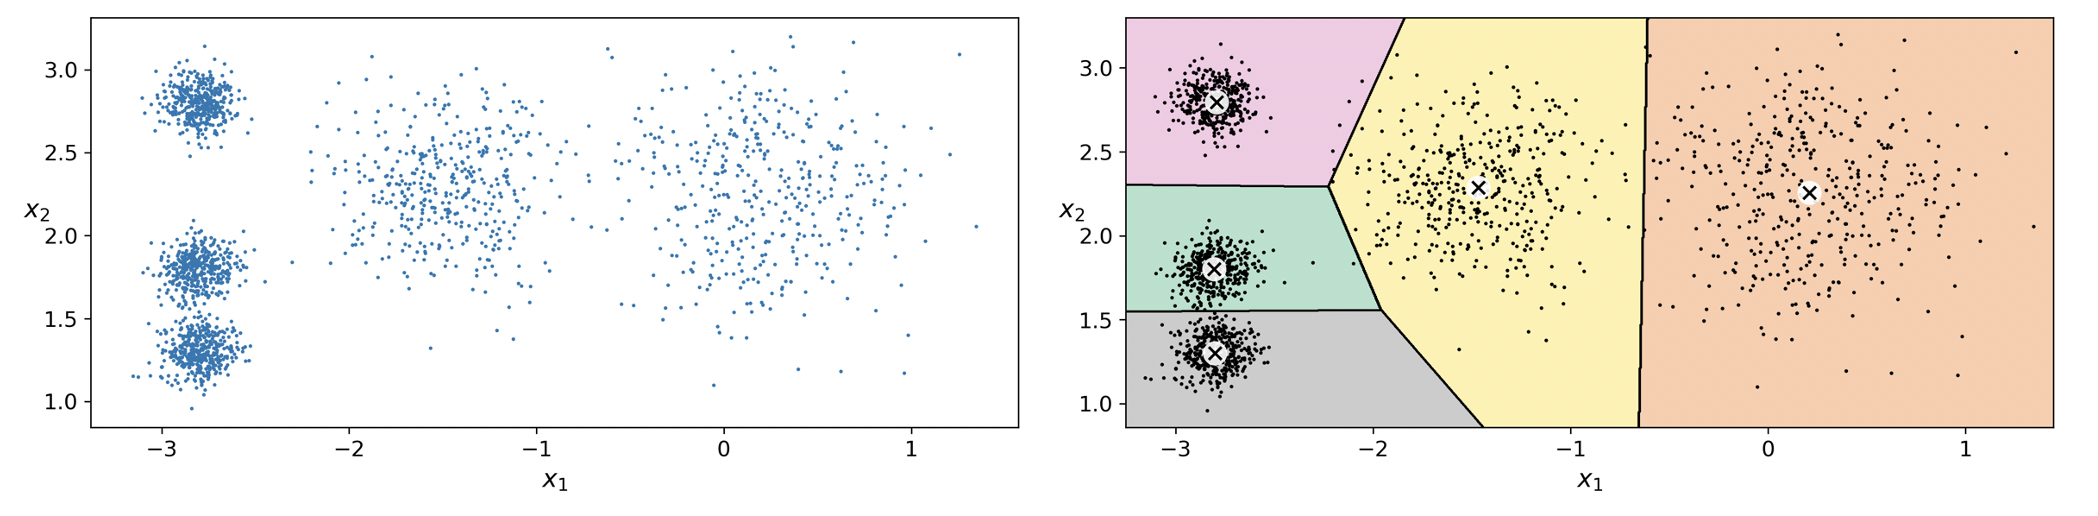
\includegraphics[width=12cm]{graphics/km_example.png}
			\caption{An example of a data distribution and the assigned cluster that k-means has predicted \cite{geron2019hands}.}
			\label{fig:km_handson_example}
		\end{center}
	\end{figure}
	
	This algorithm requires the number of clusters to get specified before initialising the model. The K-means algorithm strives to choose centroids that minimise the inertia, or within-cluster sum-of-squares criterion. The k-means algorithm divides a set of $N$ samples $X$ into $K$ disjoint clusters $C$, each described by the mean $\mu_j$ of the samples in the cluster. The means get commonly called the cluster's "centroids". However, these are not usually points from $X$, although they live in the same space. K-means gets associated with Lloyd's algorithm \cite{geron2019hands, sklearn_km}. 
	
	The algorithm has three steps. The first step chooses the initial centroids, with the most basic method being to choose k samples from the dataset $X$. After initialisation, K-means consists of looping between the two other steps. The first step assigns each sample to its nearest centroid. The second step creates new centroids by taking the mean value of all of the samples assigned to each previous centroid. The difference between the old and the new centroids get computed, and the algorithm iterates these last two steps until this value is less than a threshold. It is, in essence, repeating until the centroids do not move significantly \cite{geron2019hands, sklearn_km}.
	
	K-means scales well to a large number of samples and gets used across a broad range of application areas in many varied fields. K-means is equivalent to the expectation-maximisation algorithm with a small, all-equal, diagonal covariance matrix. When given enough time, K-means will always converge. However, this may be to a local minimum. Converging to a local minimum is highly dependent on the initialisation of the centroids. Therefore, as a result, the computation is often done several times, with different initialisations of the centroids \cite{sklearn_km}.
	
	\subsubsection{Gaussian Mixture Model (GMM)}
	
	A Gaussian mixture model is a probabilistic model that assumes all the data points get generated from a mixture of a finite number of Gaussian distributions with unknown parameters \cite{geron2019hands, sklearn_gmm}. It can get thought of that Gaussian mixture models are a generalised form of k-means clustering to incorporate information about the covariance structure of the data as well as the centres of the underlying Gaussians \cite{sklearn_gmm}. 
	
	There are multiple GMM variants, but in its simplest form for the model to get implemented it requires to know in advance the number of $k$ Gaussian distributions. At the same time, an assumption on the dataset that it gets generated through a probabilistic process (displayed in fig: \ref{fig:gmm_example}) \cite{geron2019hands}. 
	
	\begin{figure}[t]
		\begin{center}
			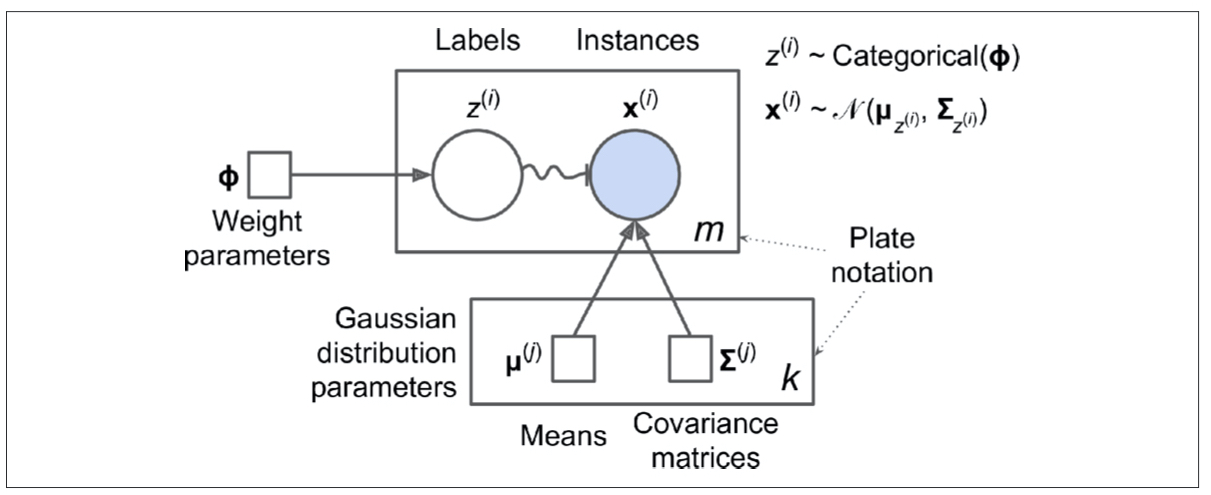
\includegraphics[width=9cm]{graphics/gmm_example.jpeg}
			\caption{An example of a GMM distribution \cite{geron2019hands}.}
			\label{fig:gmm_example}
		\end{center}
	\end{figure}
	
	GMM 's do have many advantages from its speed, and its agnostics, which is due to the algorithm only maximising the likelihood. However, GMM's do have some disadvantages. These are it suffering from singularities. This disadvantage causes the algorithm to diverge and find solutions with infinite likelihoods unless one regularises, which is due to handling of the estimates of the covariance matrices. These become difficult when the algorithm is dealing with insufficiently many points per mixture \cite{sklearn_gmm}. Another disadvantage is the algorithm dealing with several components. This disadvantage is due to the algorithm using all the features it has available. Forcing the need for held-out data to help decide on the number of components required in the absence of external cues \cite{sklearn_gmm}.
	
	\subsubsection{Neural Network (NN)}
	
	Neural Networks (NN) or also known Artificial Neural Networks (ANN), are at the very core of Deep Learning (DL). An ANN is an ML model inspired by networks of biological neurons found in our brains. However, ANN has become very different from their biological cousins that they took inspiration. ANN is what powers Google's image classifications, Apple's Siri and YouTube's video recommendation, as well as learning to beat the worlds best player at the game called Go, named 'DeepMind's Alpha Go' \cite{geron2019hands}.
	
	\subsubsection{Linear Regression}
	%%% Spec
	Linear regression is a model that aims to fit a line of best fit to the data provided \cite{geron2019hands, sklearn_lr}.  A requirement for linear regression is for a set of methods intended for regression in which the target value expects to be a linear combination of the features. In mathematical notation, if $\hat{y}$ is the predicted value. $\hat{y}(w,x)=w_0+w_1x_1+...+w_px_p$
	Across the module, we designate the vector $w=(w_1,...,w_p)$ as the coefficient and w0 as the intercept \cite{sklearn_lr}
	
	LinearRegression fits a linear model with coefficients $w=(w_1,...,w_p)$ to minimise the residual sum of squares between the observed targets in the dataset, and the targets predicted by the linear approximation \cite{sklearn_lr}. To achieve the best fit to the dataset the algorithm chooses the best overall score from the 'Root Mean Square Error' (RMSE). Therefore, to train a linear regression model, we need to find the value of $0$ that minimises the RMSE \cite{geron2019hands}.
	%%%
	Mathematically it solves a problem of the form \cite{sklearn_lr}:
	$\min\limits_{w} = ||Xw-y||^2_2$
	
	The coefficient estimates for linear regression rely on the independence of the features. When features are correlated, and the columns of the design matrix $X$ have an approximate linear dependence, the design matrix becomes close to the singular, which causes the least-squares estimate to become highly sensitive to random errors in the observed target, which in turn produces a large variance. This situation of multicollinearity can arise, for example, when data get collected without an experimental design \cite{sklearn_lr, geron2019hands}.
	
	\subsubsection{Logistic Regression}
	
	%%% Spec
	Logistic regression is an algorithm that gets used for classification and, despite its name, is a linear model rather than a regression one. Logistic regression gets also known in the literature as logit regression, maximum-entropy classification (MaxEnt) or the log-linear classifier. In this model, the probabilities describing the possible outcomes of a single trial getting modelled using a logistic function \cite{sklearn_lr, geron2019hands}. Logistic regression's model estimated probability in its vectorised form: $\hat{p}=h_\theta(x) = \sigma(x^T\theta)$ \cite{geron2019hands}.
	
	\begin{figure}[t]
		\begin{center}
			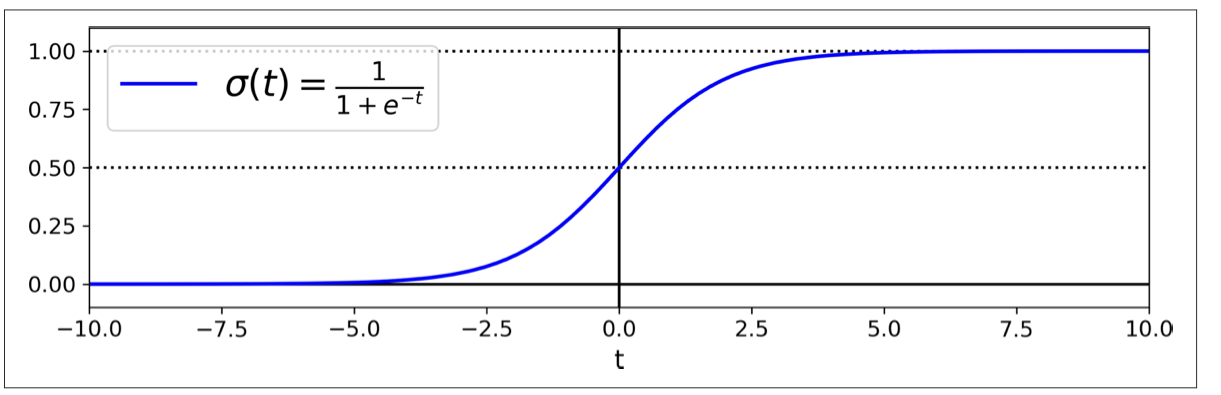
\includegraphics[width=9cm]{graphics/logistic_reg.jpeg}
			\caption{An example of a logistic regression threshold distribution \cite{geron2019hands}.}
			\label{fig:logr_example}
		\end{center}
		
	\end{figure}
	
	Logistic regression gets used to estimate the probability that an instance belongs to a particular class. If the estimated probability is greater than 50\%, the model predicts that the instance belongs to that class. If the model has predicted that the instance belongs to that class, also known as the positive class, it gets a '1' label  (see fig \ref{fig:logr_example}) \cite{geron2019hands}. Logistic regression can fit binary, One-vs-Rest, or multinomial logistic regression. That also has an optional $\ell1, \ell2$ or Elastic-Net regularisation \cite{sklearn_lr}.
	
	\subsubsection{Support Vector Machines (SVM)}
	%%% Spec
	Support Vector Machine (SVM) is a powerful and versatile ML model. The model is capable of performing linear or nonlinear classification, regression and even outlier detection \cite{geron2019hands, sklearn_svm}. This model is one of the most popular ML models and is best suited for small to medium-sized datasets. The model aims to separate the data categories by using a decision boundary, with the largest margin between them. Due to the model using a large margin to separate the data, the algorithm gets known as the 'large margin classification' \cite{geron2019hands}.
	%%%
	
	SVMs are a set of supervised learning methods and have many advantages, especially when working in high dimensional spaces. SVMs are also useful in situations where the number of dimensions is greater than the number of samples. Due to the model using subsets of the training points in the decision function, the model is memory efficient, and it is very versatile. The model is very versatile due to the different kernel functions are can be used \cite{sklearn_svm}. Although the model does have many strengths, it does also have a few disadvantages. A disadvantage is if the number of features is considerably greater than the number of data samples, then overfitting can happen. A way to overcome this is to choose different kernel functions, and regularisation of the term is crucial. Another disadvantage is that SVMs do not provide probability estimates. These estimates get calculated by using an expensive five-fold cross-validation \cite{sklearn_svm}.

	
	\subsubsection{k-Nearest Neighbour (kNN)}
		\label{seb_sec:kNN}
		
		A Neighbours-based classification is a type of instance-based learning or non-generalising learning: it does not attempt to construct a general internal model, but simply stores instances of the training data. Classification gets computed from a simple majority vote of the nearest neighbours of each point: a query point is assigned the data class which has the most representatives within the nearest neighbours of the point. Although kNN gets usually used as a classification method, it can also get used as a regression method.
		
		The k-neighbours classification in KNeighborsClassifier is the most commonly used technique. The optimal choice of the value k is highly data-dependent: in general, a larger k suppresses the effects of noise but makes the classification boundaries less distinct \cite{sklearn_knn}.
		
	\subsection{Dimensionality Reduction}
		\label{seb_sec:dd}
		
		Dimensionality reduction, or dimension reduction, is the transformation of data from a high-dimensional space into a low-dimensional space so that the low-dimensional representation retains some meaningful properties of the original data, ideally close to its intrinsic dimension \cite{geron2019hands}.
		
		Dimensionality reduction aims to reduce the dimensionality of the data. However, it also strives to maintain the meaningfulness of the data fundamentally at the same time \cite{bishop2006pattern}. The idea is to find a low dimensionality of the data but a useful representation of it. The process of dimensionality reduction is to discover the intrinsic dimensionality of the data. This reduction gets used due to some high dimensionality data actually being very low in dimensionality in reality.
		
		Dimensionality reduction aims to reduce the curse of dimensionality. The curse of dimensionality refers to various phenomena that arise when analysing and organising data in high-dimensional spaces that do not occur in low-dimensional settings such as the three-dimensional physical space of everyday experience. The expression was coined by Richard E. Bellman when considering problems in dynamic programming \cite{bishop2006pattern}.
		
		The cursed of dimensionally phenomena usually occurs in: numerical analysis, sampling, combinatorics, ML, data mining and databases. The common theme of these problems is that when the dimensionality increases, the volume of the space increases so fast that the available data becomes sparse. This sparsity is problematic for any method that requires statistical significance. To obtain a statistically sound and reliable result, the amount of data needed to support the result often grows exponentially with the dimensionality. Also, organising and searching data relies on detecting areas, within the data, where objects form groups with similar properties, for example, in high dimensional data. However, all objects appear to be sparse and dissimilar in many ways, which prevents common data organisation strategies from being efficient \cite{geron2019hands}.
		
		In a nutshell, the efficiency of many algorithms depends on the number of dimensions. However, datasets can hold a lot of redundant features. For example, not all words are useful in classifying documents like: and, or, the, of. Distance-based similarity algorithms, like K-Means and GMM, are at least linear to the number of dimensions. High dimensionality is very expensive to store, and indexing and retrieving data in high dimensional space is difficult.
	
		Principal Component Analysis (PCA) is a prevalent data reduction algorithm that gets classed as an unsupervised method. 
		
		PCA is a linear method used which will aim to reduce the data's dimensionality. It aims to do this by removing the interrelated variables while retaining as much as possible. The algorithm seeks to keeping as much variation as possible that is present within the data set.
		
		The dimensionality reduction gets achieved by transforming the data into a new set of variables. These new variables are called the principal components (PCs). These PCs are uncorrelated and get ordered in a way that the first couple of PCs retains the most amount of the variation that is present in the original variables.
		
		PCA is a decorrelation method which will linearly transform the data so that covariance values are all zeros, which, as a result, retains the components with the largest variances. While also getting rid of the components that have small variance, therefore achieving dimensionality reduction. The Eigenvectors (more below) correspond to the different principal components \cite{friedman2001elements}. 
	
	\subsection{Machine Learning in Education}
		\label{seb_sec:ml_in_learning}
	
	We will look at the styles and way ML gets currently taught to help people learn the different aspects of ML and in most cases, the overall characteristics of data science. we will be looking at classical approaches as well at any modern-day style teaching or ML educational games available. 
	
	\subsubsection{Classical Approaches}
		\label{sub_sec:classical_teach_learn}
		
		We have used the term, 'classical approach', to define methods of teaching and learning that get done in a way that is similar to what would get traditionally expected in a classroom.  Although taking into account modern takes on this approach in the forms of delivery. The classical approach is what we classify teaching and learning that gets based on a here is the knowledge, here is a task and here is the solution. Now onto the next problem, for example.
		
		Some of the most popular ways of learning ML concepts without going to university are through online learning platforms like Udemy, Coursera, edX and youTube, or you have your traditional style of lectures usually found at universities.
		
		Udemy claims to be "Improving Lives Through Learning \cite{udemy}". Udemy claims that they are the leading global marketplace for teaching and learning, having connected millions of students to skills that are needed to succeed. They have 35m learners enrolled in courses, 57k instructors, 130k courses on offer, 400m course enrollments, 110m minutes of video, 65+ languages available, over 7k Enterprise customers and they claim that 80\% of the fortune 100 companies trust them for employee upskilling \cite{udemy}. Udemy also claims that they have helped all different kinds of organisations to prepare for the ever-changing world of work. Udemy's "curated collection of top-rated business and technical courses gives companies, governments, and nonprofits the power to develop in-house expertise and satisfy employees' hunger for learning and development \cite{udemy}." 
		
		Coursera, another online teaching and learning platform, "envision a world where anyone, anywhere can transform their life by accessing the world's best learning experience \cite{coursera}." Coursera claim that you can "gain a job-relevant skill in under 2 hours" by enrolling in Guided Projects to learn job-relevant skills and industry tools. Guided Projects require a smaller time commitment, and provide practice using tools in real-world scenarios, so you can build the job skills you need, right when you need them but if you want to master a subject, it will take 4 - 6 months \cite{coursera}. Coursera are also moving in the space of online degrees. Transform your career with a degree online from a world-class university on Coursera. Our modular degree learning experience gives you the ability to study on your own schedule and earn credit as you complete your course assignments. 
		
		youTube videos can be a powerful educational and motivational tool. However, a great deal of the medium's power lies not in itself but in how it gets used. Video is not an end in itself, but a means toward achieving learning goals and objectives. Educators are increasingly using YouTube as a pedagogic resource for everything. Guidelines recommended by Clark and Mayer \cite{clark2016learning} suggest the appropriate use of any media improve learning. Suggestion means that media must get aligned with expected learning or performance outcome, reduce cognitive load, exclude simple text or graphics, be appropriate for target learner's learning literacy's Educators (and students alike). Through doing this will find that video is a significant catalyst and facilitator for classroom discourse and analysis \cite{duffy2008engaging}.
		
		While these are all popular and effective methods of teaching and learning, these methods are all purpose-driven with the content and resources getting created to deliver to the student a key concept and then moving on. This issue can get exacerbated, especially in the case of youTube, the way tutorials and lessons can get created can get very disjointed. In some cases, with different content creators teaching the same content but in different ways, can be very confusing for the learner. However, although these forms of e-learning can be beneficial, they never genuinely allowing the student to be able to just play around with learning content. Not allowing the learns to experiment with what happens if they do this or if they do that and physically see it happening, especially at a novice level. In a way, it is like a conveyer belt, everything moving along to the next thing, or in the case of learning, the next topic.
		
		Although these methods are, in their own right, all good ways to learn, they all, in essence, tell the learner here is the content and this is what it does. These methods have no way for the learner to be able just deep dive into the models and interact with them, and in most cases will only have a one use case model implemented that has minimal interaction. Therefore relying on the learner to go away and learn more about the models and then manually tweak them.
		
	
	\subsubsection{Machine Learning Edu-Games}
		\label{sub_sec:ml_edu_games}
		
		Most of the focus, in regards to ML within education, is on ML getting used to aid educational purposes, like predicting students grades, improving student retention, testing students and predicting student performance \cite{kuvcak2018machine}, rather than getting used to enable the learning and teach its concepts, especially in a Serious game context.
	
	\section{Proposed Solution}
	% Taken from spec
	The overall aim of the proposed solution is to create a fun, educating game about ML. The players will be, at the core of the solution, playing a game that interacts with different ML models. The player(s) will be manipulating the game board and data points to affect the decision boundary, or to figure out where the decision boundary or centre of the cluster is. The solution will get created by using  Pygame and will have many different algorithms in the background, doing the main game mechanics, through using libraries like SKLearn \cite{sklearn_api} and Tensorflow \cite{tensorflow2015-whitepaper}.
	
	\section{Summary and Overview of Proposed Solution}
		We have found that educational games, although they can take many forms, can only be described as so only if the games that get designed aim to help learners learn. The learning can involve certain subjects, expand concepts, reinforce development, understand a historical event or culture, or assist them in learning a skill as they play the game. Also, we have found out that a technique used to motivate plays, through extrinsic means, to behave in a certain way is called gamification. Gamification is a powerful and useful tool when implemented correctly. It is so good that it gets used almost all the time within a whole array of application. There is also a method of gamification explicitly aimed at the field of science and its wide variety of topics. This version of gamification is known as serious games. These types of gamification require the user to be able to explore and interact with the data that is on offer throughout the game. Promoting a sense of exploring and discovery.
		
		ML is a toolbox that consists of two primary methods. These methods are known as supervised and unsupervised learning. Supervised learning is when the model uses the target, also known as label, data. These allow the models to check how well they fit the data and its predictions based on the actual expected outcome of the data's target. The main goal of supervised learning is usually to do one of two things, either regression or classification. These supervised methods include linear regression, logistic regression and neural networks.
		
		In comparison, unsupervised learning's models expect there to be no labels to the data. So the models will fit and predict the data based on the model selected actions. These actions can be clustering, data association and dimensionality reduction. Some of these algorithms include k-means, PCA.
		
		The proposed solution will aim to create an application that will incorporate elements of gamification and serious games, as well as actual gaming mechanics to create a fun and engaging game. This game will be about ML while providing aspects of teaching and learning. The teaching and learning will be in the form of learning reading content, quizzes and exploration through the game by interacting with the models.
	\chapter{Design}
	\label{chap:methodology}
		
	%The university has subscriptions to a vast number of major academic journals spanning a wide range of subject areas. By accessing the internet from a university network connection (Eduroam or Ethernet), the paywalls of many journals will simply vanish without any need for login credentials.

	\section{Overview of Application}
	%	When you are working from outside of the university then connecting to an on campus machine via remote desktop (RemoteDesktopProtocol, TeamViewer, ect) or via port forwarding (ssh, ssh tunnel, ect) can allow you to access papers that would otherwise be behind a paywall. 
		
	%	If you do not have individual access to a machine that is exposed for ssh on the university network you can always use the computers in Linux Lab CF204\footnote{One caveat of using computer lab machines for remote tunnelling is that a environmentally conscious student who has worked late in the computer lab might choose to switch off the machine you were using...} for the purpose of setting up an ssh port tunnel to proxy your internet through. These machines have fixed IPv4 addresses and respond to ssh using your student account credentials. While in use your internet will be routed\footnote{Painfully slowly.} to the university and then out to the internet, granting you transparent access to journals without a paywall.
	The application has three main segments. These segments are a game area, a learning area and an exploring area. Each area's intension is to help support the user learning and understanding of the different machine learning models using a blend of exploration, fun and interactivity as well as a more traditional teaching a learning style of quizzes and learning reading material. Although each segment has its core task, together they help give the user a rounded learning experience while creating gamification incentives to come back and use the application some more.
	
	With the application being about the user interacting with data, and placing (splashing) the data points around a game board, we decided upon the title "Data Splash". With the title 'Data Splash" agreed upon, a beach and sea themed colour pallet got chosen. The pallets colours contained blue, yellow, turquoise and orange. However, additional colours got used to aid the colour pallet selected, and these colours involved grey and red.
	
	All the screens had a similar layout, with a title banner image at the top, the content in the middle and the buttons in the bottom general area. The only screens that are different are the main menu screen and the coming soon splash screen. The main menu did follow a similar structure, but the main content was the buttons, which get presented in a horizontal stage manner.
	
	Whenever a model or educational content got made available to the player, this content was the main focus to the screen. Therefore always making sure that the user's attention was on interacting with the model or learning about them. Unless like in the Free Play area, both learning and model interaction was available, equal weighting occurred given to allow focus on interacting and learning about the machine learning models.
		
	%\subsection{Design}
	
	%\begin{figure}[t]
	%	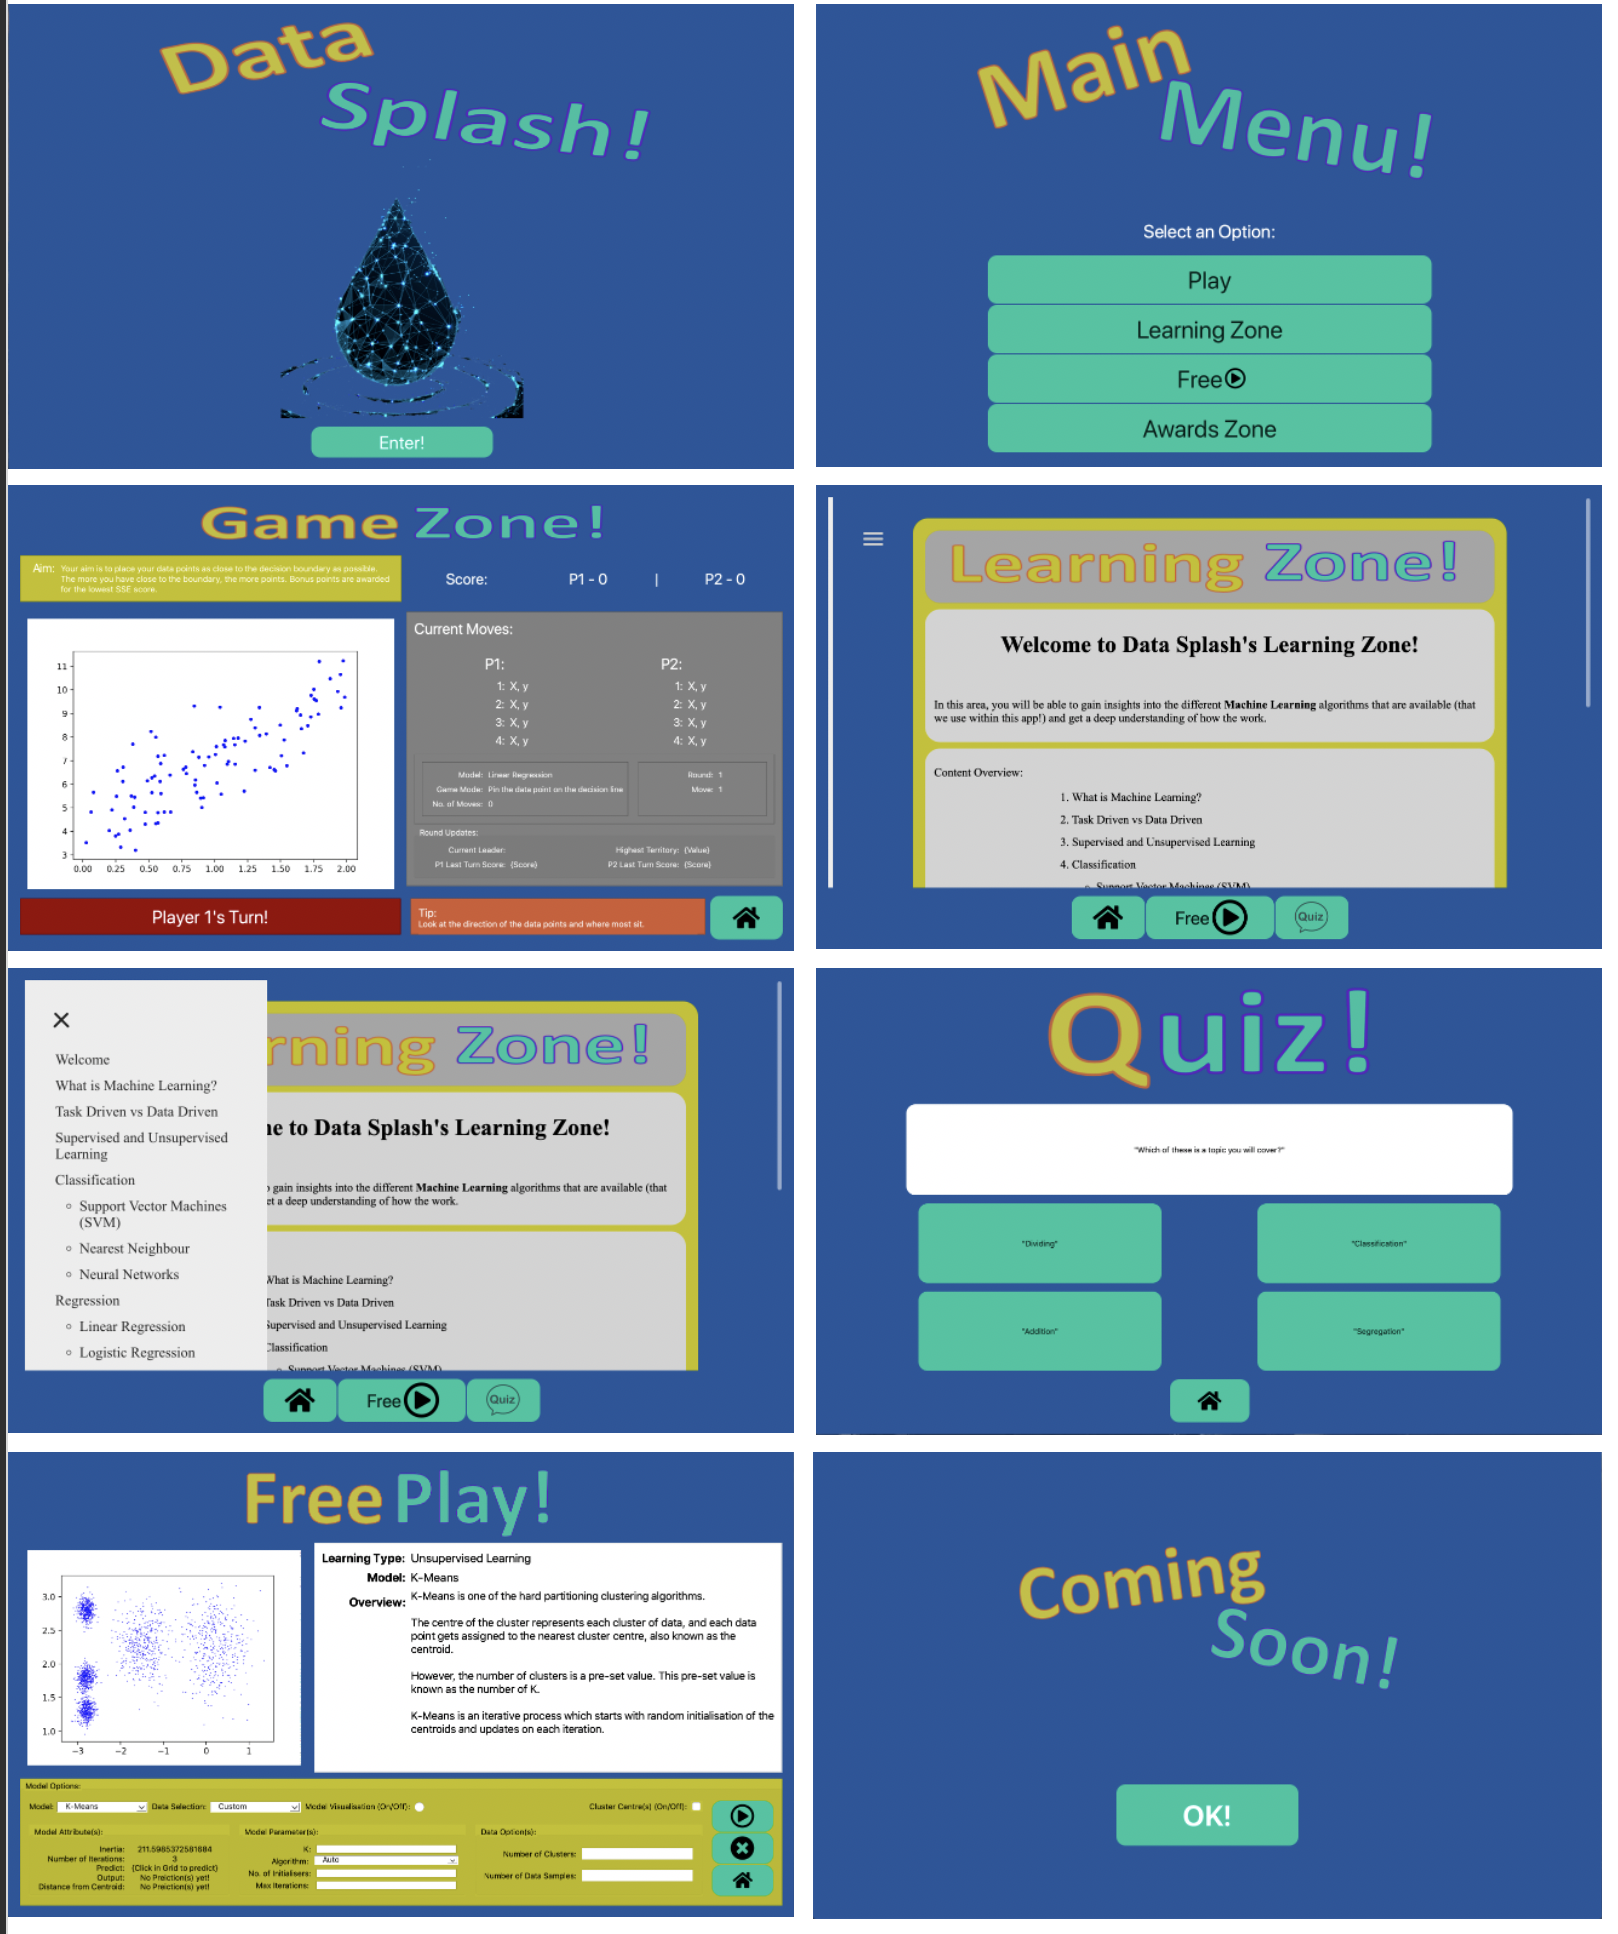
\includegraphics[width=15cm]{graphics/ui_screens.png}
	%	\caption{Each screen available within the application.}
	%	\label{fig:ui_screens}
	%\end{figure}
	
	
	
		
		
		
	\section{Overview of Specific Game Components}
		\label{sec:overview_game_components}
		
	
	\subsection{Main Menu \& Modular Design}
	\begin{figure}[t]
		\begin{center}
			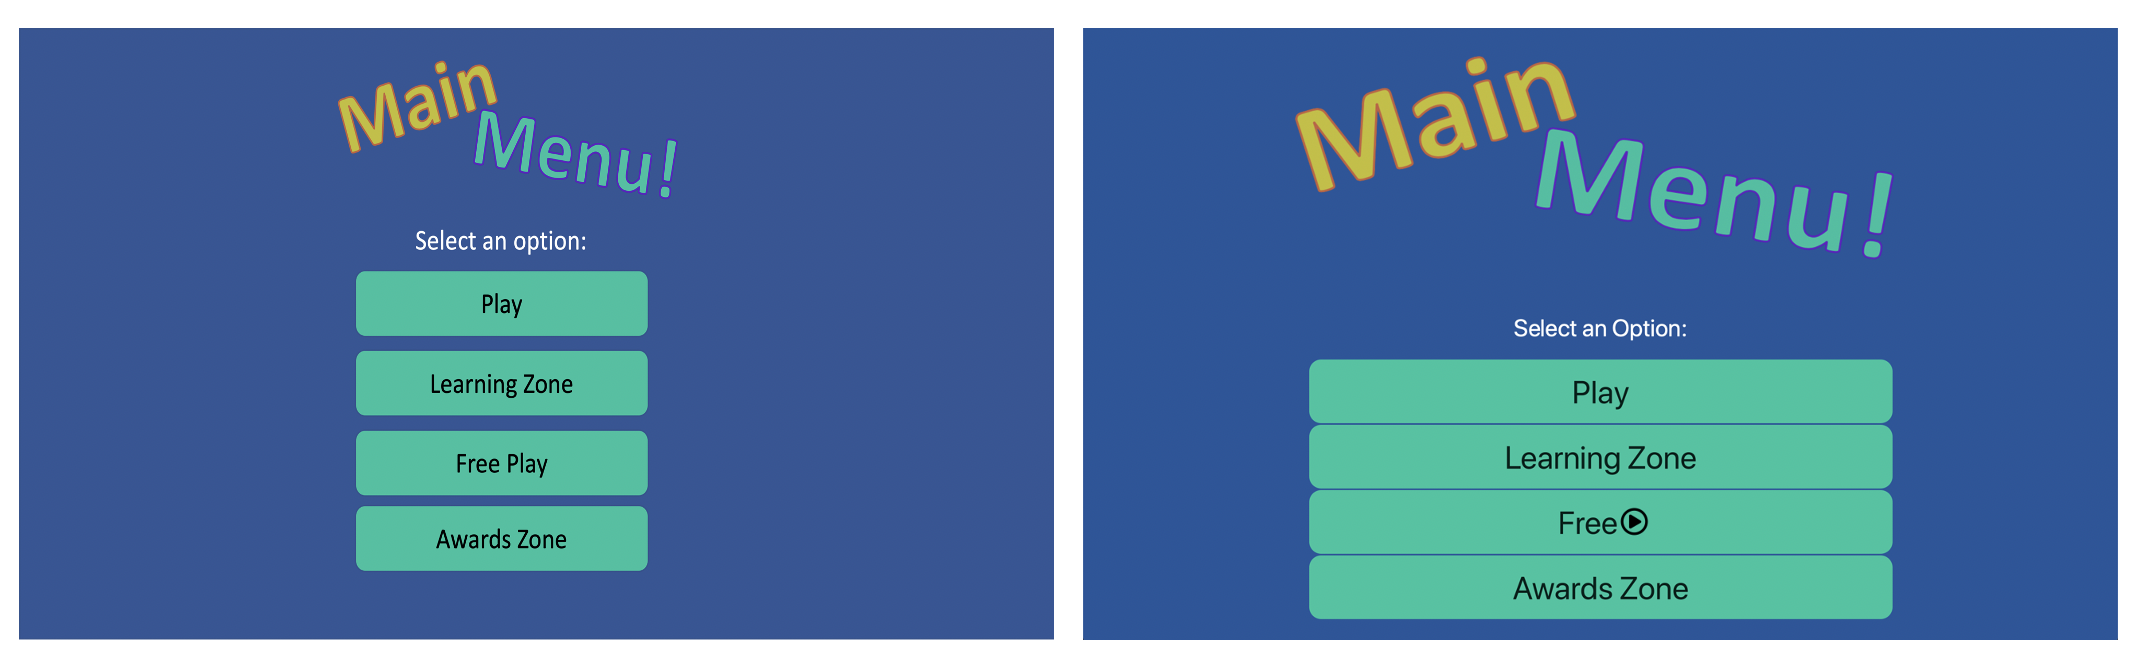
\includegraphics[width=11cm]{graphics/main_menu.png}
			\caption{A comparison of the main menu's designed screen UI and the final implmented UI.}
			\label{fig:ui_mm}
		\end{center}
		
	\end{figure}

	The main menu is the central hub of the application. This area allows the player to be able to navigate to whatever place they chose within the application. They design to this window stayed very close to the original design (see fig: \ref{fig:ui_mm}), the only main change was that the buttons ended up being longer than initially designed.
	
	The application got designed in a modular way, by creating the application this way allowed for code to be reusable, especially in regards to the machine learning models. Therefore allowing the game area and the free play zone to be able to use the same models, as well as use the same functions. However, these functions work differently based on the model that gets selected. 
	
		
	\subsection{Game Arena}
	
		The 'Game Zone' was the critical area that intended to use game mechanics, and gamification, to help drive the learning of the different machine learning models. The game zone is an area that allows one on one (player vs player) game action. The game gets conducted over three rounds, with each game round having a random model generated for the players to interact. At the time of writing this report, the available models for the game zone are Linear Regression and K-Means. A Neural Network got implemented with game mechanics, but due to time restrictions, we were unable to add them to the application in time. As the research suggested, having a competitive nature to the game creates desired external motivation for the player to learn more about the ML models, to be able to have a better chance of winning. A running score is presented to the players to let them know who won the previous round and who is currently winning. The multiple forms of game stats allow the players to have an idea of what is needed to win the game potentially through using sport like game mechanics to add the layer of progress updates continuously, to create that sense of competitiveness and external motivation. Even though there were only two models implemented fully into the game, these models offered several different gaming outcomes. For example, each model had multiple datasets which would get selected at random. In terms of K-Means, a random dataset would get generated each time or a preselected dataset, but the k value would change and be a random number. So even though the dataset was a k value of 2, the challenge would be added by not knowing what k value was given to the model for the user to predict the centroid value. 
		
		\begin{figure}[t]
			\begin{center}
				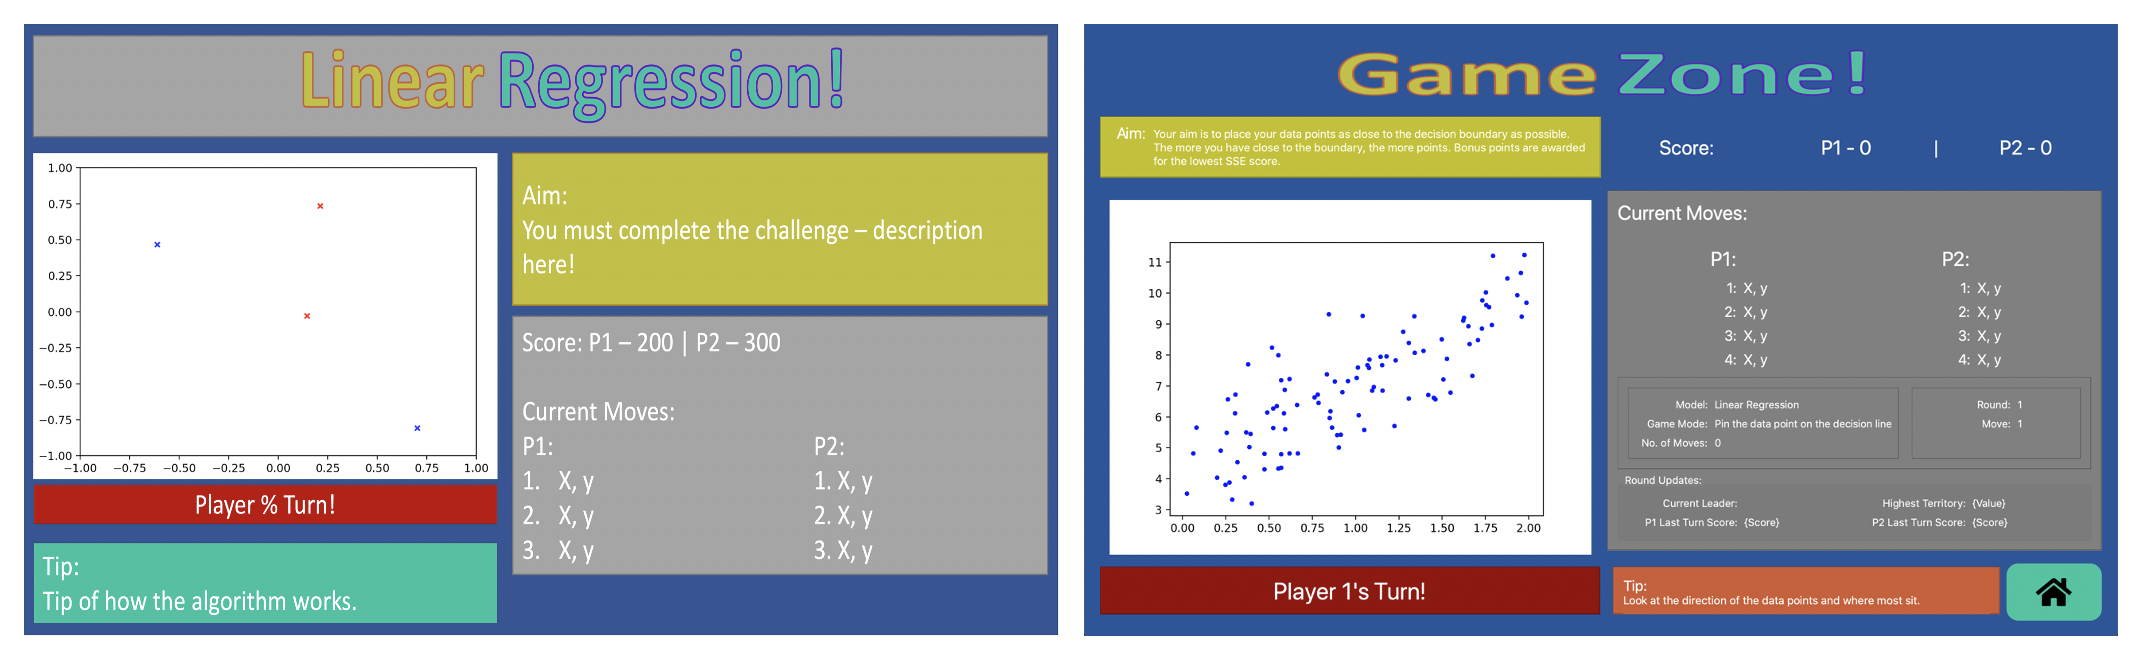
\includegraphics[width=11cm]{graphics/game_zone.png}
				\caption{A comparison of the game area's designed screen UI and the final implmented UI.}
				\label{fig:ui_ga}
			\end{center}
		\end{figure}
		
		
		We selected K-Means and Linear Regression to be implemented first due to them both having a similar game mechanic intention. Linear Regression was using the SSE metric value as the deciding factor to determine the game's winner, while K-Means was using the model's metric value of the euclidean distance to do the same thing. The neural network uses a territory-based mechanic, and this intention was to add variety in not only the models but the game times. Challenging the players understanding of how different models work.
		
		With having multiple models available, as well as getting the models and their datasets randomly selected each time, this allows the game to feel fresh each time and not have a set pattern of motions. Therefore, by creating a sense of game mode uncertainty or randomness will keep things fresh. Thus, ultimately making sure that a critical mechanic of gamification, which is replayability, be achieved.  
		
	
	\subsection{Learning Zone}
	
	The learning zones aim is for the user to do the principal amount of learning about the different machine learning models. The main content gets presented to the user by using a web browser widget. This widget would link to a multipage HTML website that holds all the content about the different models with pictures. We decided to use this combination as it allowed us to update the learning content and add new content as we went along, enabling the main functionality not get affected. Also, it avoided unnecessary long developing time, because of the updates and the new content, forcing the redesign of the game screen. 
	
	With the teaching and learning getting conducted through text and images on the webpages, we decided to add a quiz. The quiz was to allow the user to assess how much they have learnt. A useful tool used by teachers to evaluate students learning is different questioning techniques. In an attempt to allow the users to test their subject knowledge, but keeping everything in a game-like manner, a quiz was implemented. The quiz, with not only challenging the user but also offers an overall score allowing the user to know how they did and will enable a form of competition to happen and also let the use sense a way of progression by observing their performance improving.
	
	An option available to the user is not only to quiz themself but also to have the ability to go straight to the Free Play area. When the user selected this option, the model that the user has been learning about will be preloaded into the screen, allowing them to be able to interact with it. We decided to do this as although you can learn a lot about a topic by reading about it, an effective way to truly learn about something is to be able to interact with it and see what is happening by, in essence, trying to break it in a sort of way.
	
	\begin{figure}[t]
		\begin{center}
			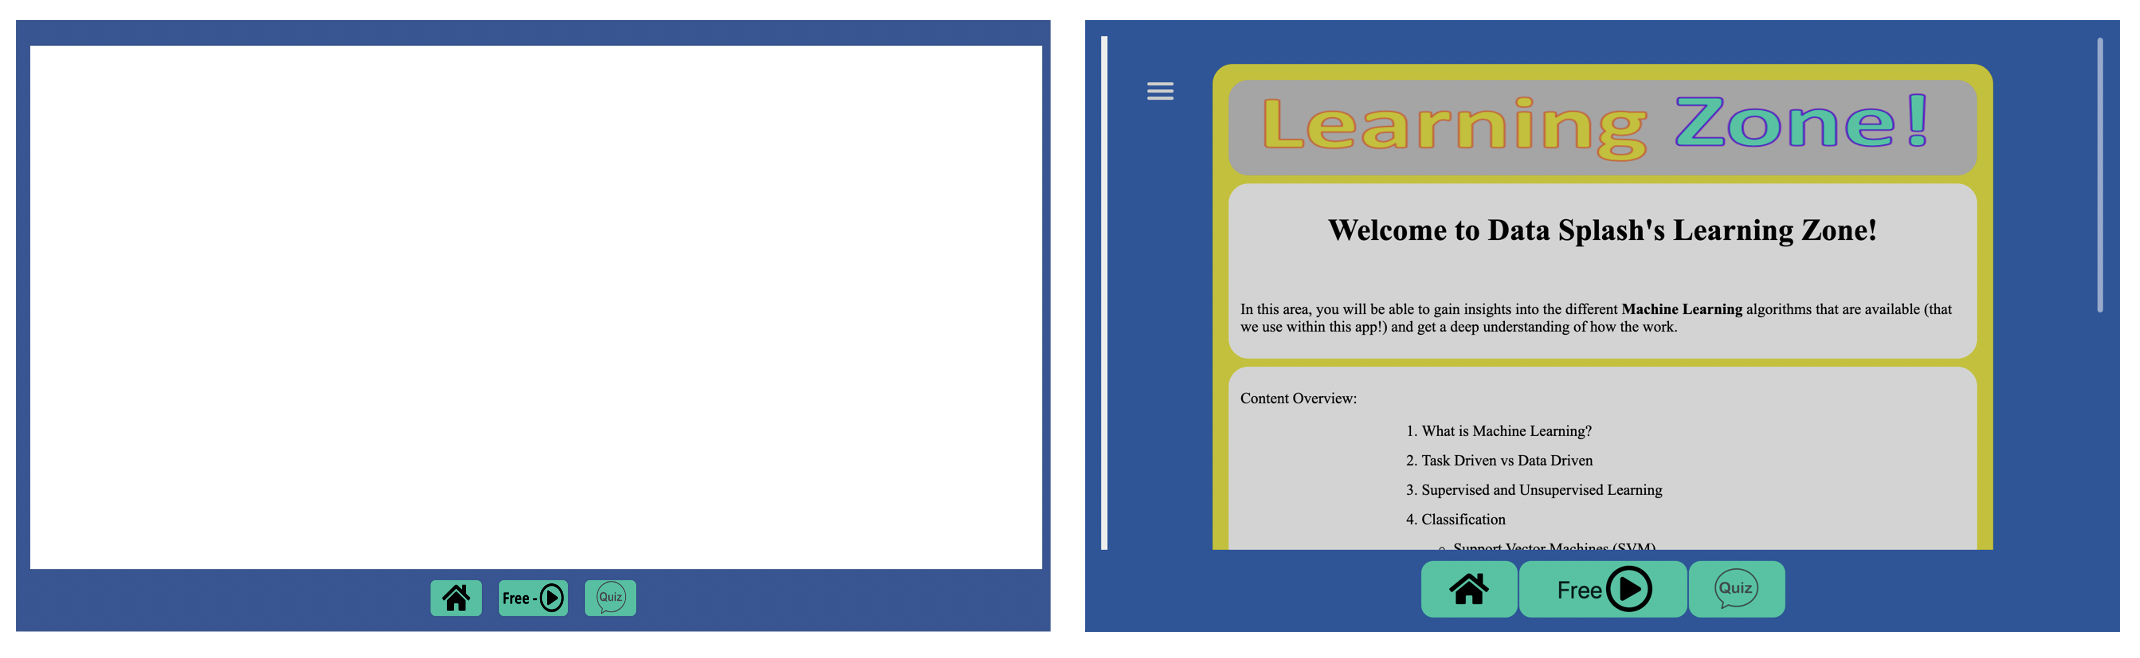
\includegraphics[width=11cm]{graphics/learning_zone.png}
			\caption{A comparison of the learning zone's designed screen UI and the final implmented UI.}
			\label{fig:ui_lz}
		\end{center}
	\end{figure}
	
	\subsection{Free Play}
	
	The free play area is where the serious gamification style gets implemented. This area intends to allow users to be able to interact with the ML models. Initialise not only the models but also set the type of data they want to have displayed and even add additional data points. By allowing the user to add extra data points to the existing data, it will update the model and, for example with Linear Regression, will show to the user, how the additional data points will affect the model's decision making.
	
	\begin{figure}[b]
		\begin{center}
			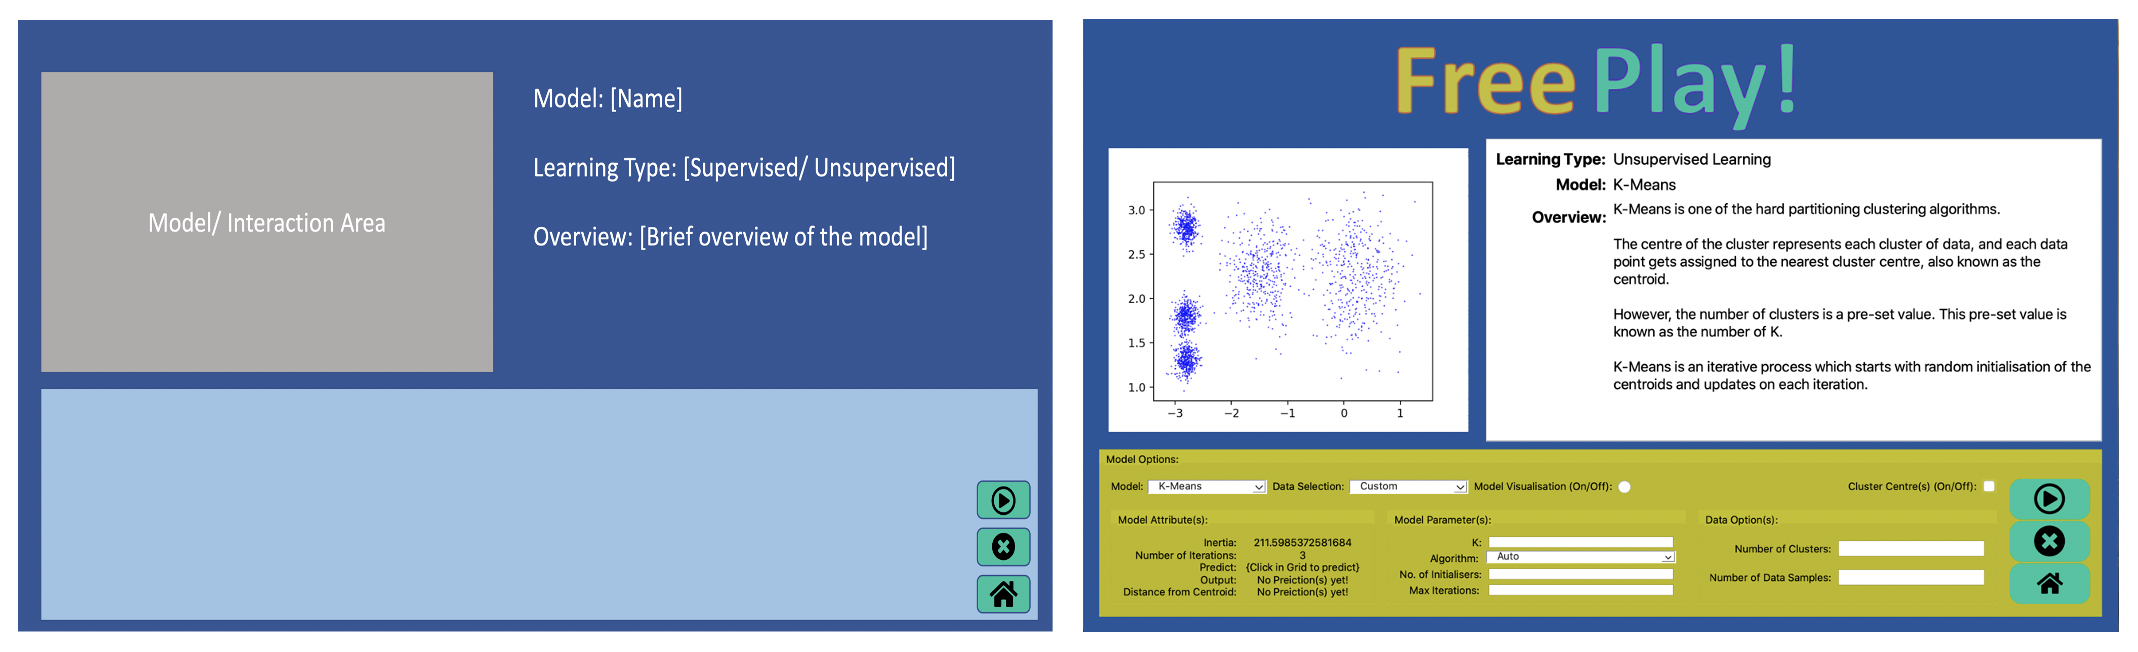
\includegraphics[width=11cm]{graphics/free_play.png}
			\caption{A comparison of the free play's designed screen UI and the final implmented UI.}
			\label{fig:ui_fp}
		\end{center}
	\end{figure}
	
	The most interactive model's within the FP area, at current, are the models Linear Regression, K-Means, LDA and Neural Networks. However, the models GMM and SVM are also available, but with less interactivity as the others. K-Means allows the user not only to select different data sample but also select how many clusters they want the dataset to have, but also independently change the k value of clusters. We decided upon this feature to allow the user to see, knowing how many k clusters the dataset has, to see by changing the algorithms k value how is that then affected on the dataset with its outcome. The user can click within the Matplotlib widget and see what the data points prediction values are as well. We decided to use a click in the widget functionality, as we believed having the user input x and y coordinates would make the UI look cumbersome and add unneeded fiddliness for the user, trying to figure out the exact values they want. Linear regression allows the player to be able to make predictions, as well as additional data points allowing them to see how the data can be altered and manipulate and what implications that has on the models fitting. However, Linear Regression does not provide as much control for the intricacies of the model compared to K-Means, but it does offer the parameters and outputs that the model has. For example, the intercept and the coefficients to the model. Neural Networks offer slightly less control to the user compared to the other two, but more than LDA but both of them have fully interactive models. SVM and GMM, on the other hand, do not. GMM allows the user to switch its predictions on and off, but SVM just shows the models predictions. These got implemented to help with understanding the content from the learning zone, but we decided to focus on the other models due to them having more game-like features to get used in the game area.
	
	There were intentions for the Learning Zone to also provide example code for the user, after specific gamification actions, for example getting full marks in the quiz, were completed as bonus rewards. The intention of this was to allow the users to not only learn about the code but also see the code, to help see the mechanics in it. However, due to time restrictions and certain gamification features not being implemented, this additional feature was not added at this point.
	
	
	
	\subsection{Awards Zone}
	
	\begin{figure}[t]
		\begin{center}
			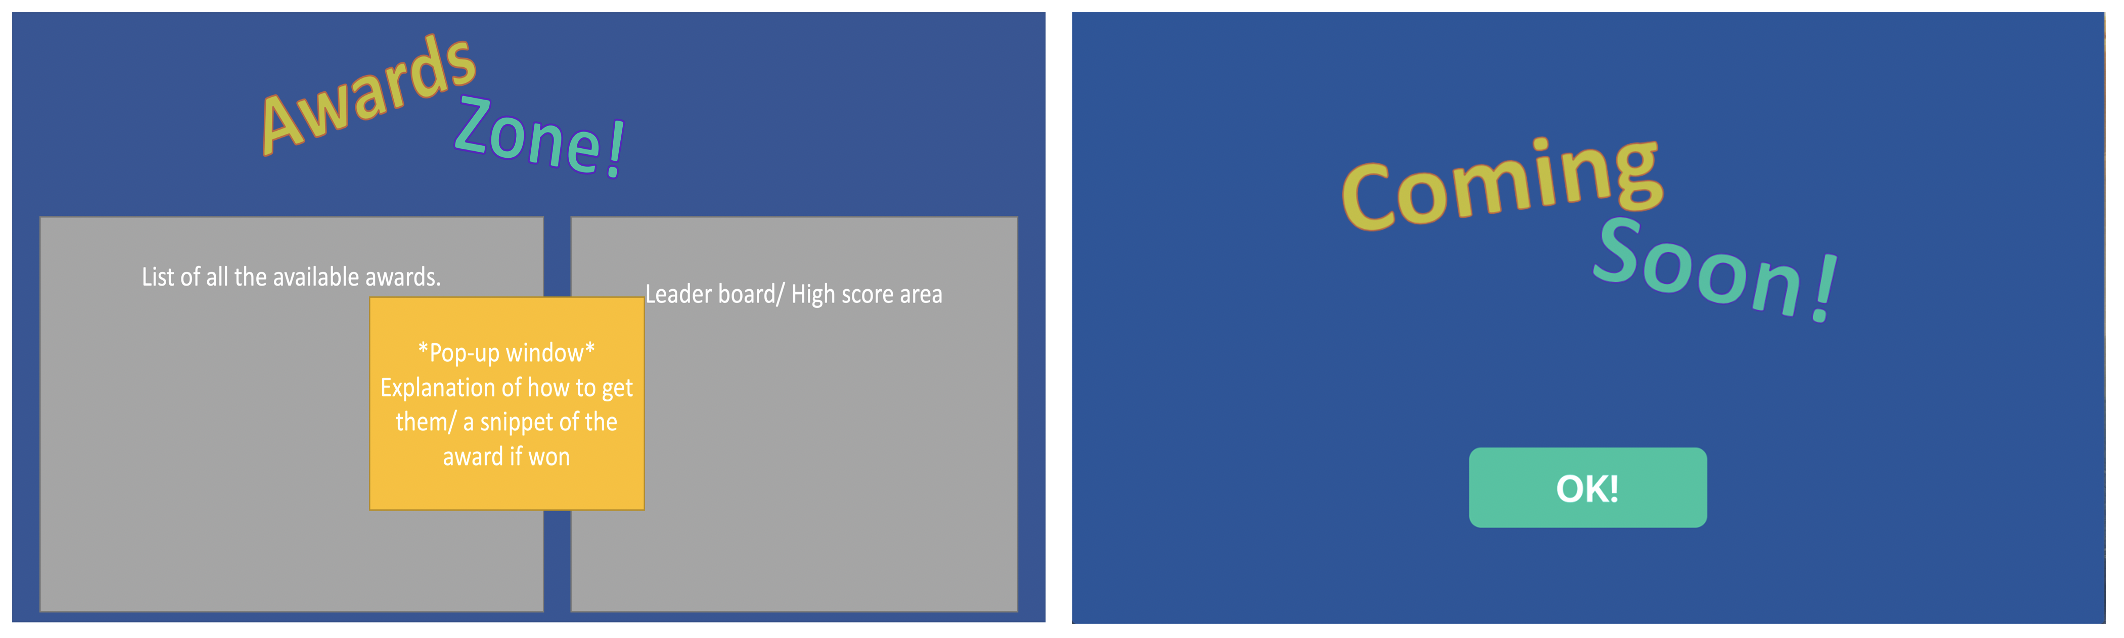
\includegraphics[width=11cm]{graphics/awards_zone.png}
			\caption{A comparison of the awards zone's designed screen UI and the final implmented UI.}
			\label{fig:ui_az}
		\end{center}
	\end{figure}
	
	
	The achievement area has just a title, coming soon image and a button. Once the button gets pressed, it will return the player to the main menu. This area intention was to be the central hub of where all the gamification elements of badge unlock and progress, would be displayed to the user, giving them instant feedback on unlocked prizes and game modes,  as well as hints on what to do to unlock additional features. However, due to time restrictions, this was unable to be implemented within the application. The idea was to allow the users to see how or what affects the models, from little changes to significant changes like changing the number of clusters in k-Means or the main algorithm being used to fit the clustering data. The intention was to allow the user to get hands-on with the different models, to see what they have learnt from the learning zone in motion, and also try out strategies for the game zone. 
	
	The models had three data settings, a custom one and two pre-generated datasets. The pre-generated data sets allow the user to be able to change the features that are used, assigning news features to the X and y-axis.
	
			
	\section{Evaluation of Application}
		\label{sec:app_evaluation}
	
		To gain a deeper understanding of the application, for its effectiveness and the general overall thoughts from other peoples views, a user study got conducted. The user study involved participants in interacting with the application and then fill in an online questionnaire about what they thought of it. However, due to the coronavirus pandemic, the study got done all remotely.
		
		The user study involved six of participants and got done in a quantitative style, using questionnaires of a range scale. This style of questions got decided upon due to the inability to ask the candidates follow-up questions. The participants got asked to install the application and then spend a minimum of 20 minutes interacting with it. After they had spent a minimum of 20 minutes on the application, they then needed to complete a questionnaire. The questionnaire consisted of [number of] questions with the questions either a range option style question of 1 to 5 or a short paragraph explanation. The questionnaire got conducted using Google Forms, which allowed us to have all the responses appear in a spreadsheet. Therefore, allowing reflection on the user's opinions more accessible.
		
	\chapter{Methodolgy and Implementation}
	\label{chap:implementation}
	
	\section{Tools}
	
	\subsection{Programming Languages}
	
	For the implementation of our application, three primary programming languages deemed to be best suited for development. Apple's Swift programming language \cite{swift} got considered early on, due to the author's familiarisation with the programming language. The programming language gets used for creating applications for Apple's mobile and desktop operating systems, and with 1.5 billion \cite{9to5mac} iOS devices in circulation, that was a lot of potential users. Additionally, Apple's iOS devices are prevalent within most educational settings, with Apple's iPad being one of the primary go-to devices. However, due to the language not supporting key frameworks required, or providing similar alternatives, the decision to not use this language got made. 
	
	We then got presented with three main options to use, Python, R and HTML, CSS and JavaScript.
	
	Python is a very popular programming language \cite{wired_python, sof_dev_servay20}, it is fast, easy-to-use, and easy-to-deploy programming language that gets widely used to develop scalable applications. Examples include YouTube, Instagram, Pinterest and SurveyMonkey \cite{hackr.io}. The Python Software Foundation state that Python is a high-level, object-orientated (OOP), interpreted language with dynamic semantics. Due to the language being a high-level, it has many built-in data structures. These features, along with the dynamic typing and dynamic binding together make Python attractive to development teams working in a Rapid Application Development (RAD). As Python is an extracted level above the C language \cite{sto_cpython}, Python can get used as the glue that connects existing components, as well as being able to be used as a scripting language \cite{python_desc}. Python gets considered to be easy to learn the language due to its high readability and is recommended by many exam boards as the language to use for teaching Computer Science at GCSE and A-Level level \cite{list exam boards here}. Python's simple and easy to learn syntax emphasises on readability, which, as a result, reduces the cost of program maintenance \cite{python_desc, pyqt_rbc}. 
	
	Python gets compared to a lot of other languages. However, due to the requirements and expectations of the application, we will compare it to other similar style applications that can potentially do a similar job. These being Java, JavaScript and C++. In general, the choice of the programming language to use is many other real-world constraints, for example, financial cost, availability, training and even personal preferences and attachments. However, we will focus on language issues for the comparisons.
	
	\begin{figure}[t]
		\begin{center}
			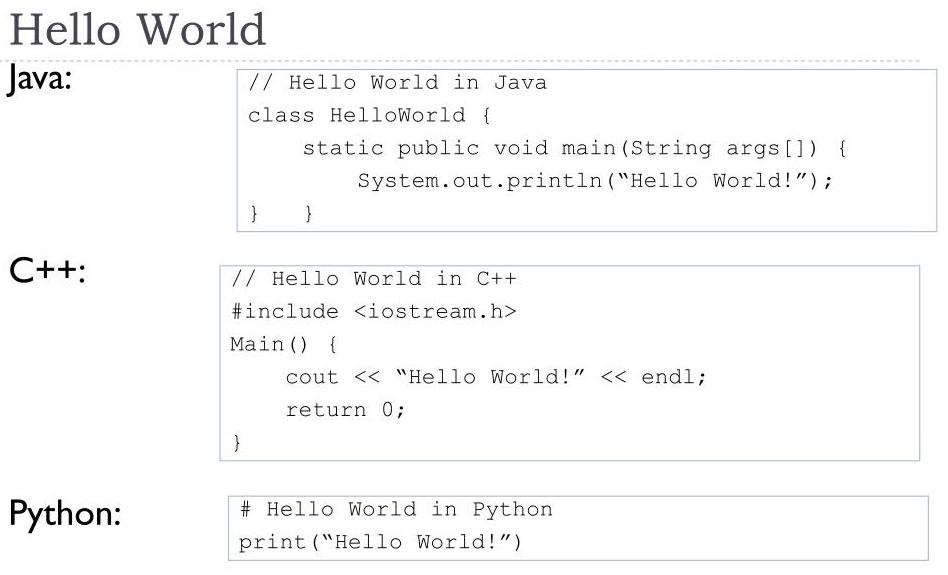
\includegraphics[width=8.5cm]{graphics/python_vs_java_vs_c++.jpg}
			\caption{A comparison between Java, Python and C++ to print an output to the console. \cite{py_ja_c++}}
			\label{fig:py_java_c++}
		\end{center}
	\end{figure}
	
	In comparison to Java, Python programs will typically take 3-5 times quicker (See fig: \ref{fig:py_java_c++}) to develop but will have a slower run time. The time difference gets attributed to Python's built-in data types and its dynamic typing \cite{python_comparison}. As Java gets better characterised as a low-level implementation language, this would be the language of choice if application execution speed was the deciding factor. If this is not a factor, then there is no real benefit over Python.
	
	What gets said about Java is also the same when comparing C++ to Python. It is often 5-10 times shorter than equivalent C++ code. Anecdotal evidence suggests that one Python programmer can finish in two months what two C++ programmers cannot complete in a year. Python shines as a glue language, used to combine components written in C++ \cite{python_comparison}.
	
	In comparison to JavaScript (JS), Python's 'object-based' subset is very similar to JS. Python supports a programming method that uses simple variables and functions, similar to JS, that do not need class definitions. However, Python also supports writing for much larger programs, which leads to more reusable code by using an accurate OOP way while with JS, that is all that it can do \cite{python_comparison}.
	
	Another language that presented itself to us was the R language. R is a language and environment for statistical computing and graphics. It is a GNU project which is similar to the S language and environment which was developed at Bell Laboratories (formerly AT\&T, now Lucent Technologies) by John Chambers and colleagues \cite{r_project}. Many users think of R as a statistics system \cite{r_project}. Academics and statisticians have developed R over two decades. There are around 12000 packages available in CRAN (open-source repository). The wide variety of library makes R the first choice for statistical analysis, especially for specialised analytical work \cite{r_vs_py}.
	
	R provides a wide variety of statistical (linear and nonlinear modelling, classical statistical tests, time-series analysis, classification, clustering) and graphical techniques, and is highly extensible. One of R's strengths is the ease with which well-designed publication-quality plots can be produced, including mathematical symbols and formulae where needed \cite{r_project}. The cutting-edge difference between R and the other statistical products is the output. R has fantastic tools to communicate the results. Rstudio comes with the library knitr. Communicating the findings with a presentation or a document is easy \cite{r_vs_py}.
	
	R and Python are both open-source programming languages with a large community. New libraries or tools are added continuously to their respective catalogue. R is mainly used for statistical analysis, while Python provides a more general approach to data science.
	R and Python are both state of the art in terms of programming language oriented towards data science. Learning both of them is, of course, the ideal solution. R and Python requires a time-investment, and such luxury is not available for everyone. Python is a general-purpose language with a readable syntax. R, however, is built by statisticians and encompasses their specific language \cite{r_vs_py}.
	
	Python can pretty much make the same tasks as R: data wrangling, engineering, feature selection web scrapping, creating an app, for example. Python is a tool to deploy and implement machine learning at a large-scale. Python codes are easier to maintain and more robust than R. Years ago; Python did not have many data analysis and machine learning libraries. 
	
	Recently, Python is catching up and provides cutting-edge API for machine learning or Artificial Intelligence. Most of the data science job can get done with five Python libraries: Numpy, Pandas, Scipy, Scikit-learn and Seaborn \cite{r_vs_py}.
	
	Python, on the other hand, makes replicability and accessibility easier than R., if we need to use the results of our analysis in an application or website, Python is the best choice \cite{r_vs_py}.
	
	In 2019 there was an active number of 26.66 billion devices attached to the internet \cite{securitytoday, statista_iot}, with an estimation of 35 billion in 2021 \cite{securitytoday} and by 2025 75.44 billion \cite{statista_iot}. Experts estimate that the IoT device market will reach \$1.1 trillion in 2026 \cite{securitytoday}. Every Second 127 new devices get connected to the world wide web \cite{securitytoday}.
	
	With so many devices on the internet, an important consideration we had was to make the application web-based. By creating the application for the internet, this would allow potentially many more people to be able to access the application and interact with the different ML models. 
	
	JS gets regarded as more of the language of the world-wide-web \cite{web_foundation}. It got initially designed to be used client-side in a web browser. However, it has in more recent years started to branch out and be able to be used to create applications on, not only the front end of the web but also desktops, servers and mobile platforms natively. For example, React Native, Node.js and TypeScript. JavaScript is also incredibly useful, allowing developers to be able to create apps with audiences in the millions quickly \cite{js_springboard}.
	
	The decision on what language to use we a close call between Python and JavaScript, this was due to the massive amounts of libraries that were on offer and the support communities that were in place. With both being open source and both having essential libraries available to interact with machine learning models and visualisation tools, both could have been a perfect fit for the intended application. However, we decided upon using Python. Python was chosen based on it being the go-to language for anything machine learning related, and its ability to be able to be used multiplatform on desktops or mobile devices. Python supports modules and packages, which encourages programs to be developed modularity and therefore allows code to get reused. The Python interpreter and the extensive standard library are available in source or binary form without charge for all major platforms and can get freely distributed \cite{python_desc}. There was also an additional factor that the author was more familiar with Python and its required libraries compared to the libraries that will get required for using JavaSript.

	There was the additional decision to use HTML and CSS within a small part of the project, the 'Learning Zone', based on the quickness of being able to create and host the webpages containing the learning content. It was allowing the learning content to evolve without having any impact on the overall development of the main application, allowing the learning content to be an individual entity within the main application.
		
		
	\section{Frameworks}
	
	\subsection{GUI Framework}
	
	With the nature of the application, we needed to make the application have a Graphical User Interface (GUI). Having a GUI allowed the learning to be a lot more hands-on and allow the players to see what is happening within the models, especially when they interact with them.
	
	Therefore, due to the GUI requirement, three GUI libraries presented themself to us. These were Pygame, PyQT5 and Tkinter.
	
	Pygame is a free, open-sourced library. Released under the LGPL licence, Pygame is a set of Python modules designed for writing video games. Pygame adds functionality on top of the standard Python library. Pygame allows the user to create fully featured games and multimedia programs in the python language \cite{pygame_wiki}.
	
	Pygame is highly portable and runs on nearly every platform and operating system, and it gets downloaded millions of times \cite{pygame_wiki}. 
	
	With the main aim of the application to be a game, Pygame was a strong contender. It was providing modules that can handle a lot of the key gaming mechanics and multiple screen switching. However, it lacked some key features that were deemed essential for the application. It was unable to provide a library that could create interactable graphs to be used as data inputs for the models and be able to render HTML and CSS content for the Learning Zone. Therefore reducing the amount of flexibility, it got decided upon for using HTML and CSS for the learning content. Therefore, meaning that all the content would need to be hardcoded. If any changes were needed, a significant transformation would need to happen to the overall code, instead of just changing the web content.
	
	PyQt is a set of Python v2 and v3 bindings for The Qt Company's Qt application framework and runs on all platforms supported by Qt including Windows, macOS, Linux, iOS and Android. PyQt5 supports Qt v5. PyQt4 supports Qt v4 and will build against Qt v5. The bindings are implemented as a set of Python modules and contain over 1,000 classes \cite{pyqt_rbc}. PyQt brings together the Qt C++ cross-platform application framework and the cross-platform interpreted language Python.
	
	Qt is more than a GUI toolkit. It includes abstractions of network sockets, threads, Unicode, regular expressions, SQL databases, SVG, OpenGL, XML, a fully functional web browser, a help system, a multimedia framework, as well as a rich collection of GUI widgets. Qt classes employ a signal/slot mechanism for communicating between objects that is type safe but loosely coupled making it easy to create re-usable software components \cite{pyqt_rbc}. Qt also includes Qt Designer, a graphical user interface designer. PyQt is able to generate Python code from Qt Designer. It is also possible to add new GUI controls written in Python to Qt Designer \cite{pyqt_rbc}. PyQt combines all the advantages of Qt and Python. A programmer has all the power of Qt but can exploit it with the simplicity of Python \cite{pyqt_rbc}.
	
	Tkinter is the third option. Tkinter commonly comes bundled with Python, using Tk and is Python's standard GUI framework. It is famous for its simplicity and graphical user interface. It is open-source and available under the Python License \cite{data_camp_gui}.
	
	Tkinter is Python's de-facto standard GUI (Graphical User Interface) package. It is a thin object-oriented layer on top of Tcl/Tk. Tkinter is not the only GuiProgramming toolkit for Python. It is however the most commonly used one. CameronLaird calls the yearly decision to keep TkInter "one of the minor traditions of the Python world \cite{py_tkinter}." Tkinter supports functionality with Matplotlib, with Matplotlib offering libraries to allow handling the backend of the graph creation interacting with the GUI library. However, unlike QT, Tkinter does not support any GUI designer. Therefore the GUIs will have to be created programmatically, which will give more control, might involve more of a learning curve and potentially more time to implement in the initial stages.
	
	After reviewing the different GUI libraries, PyQt was the decided library to use. We believed it would give us the ability to have 
	
	
	\section{Packages}
	\label{sec:packages_used}
	
	In order to create the application, there are several Python libraries required. The main one being PyQT5 \cite{pyqt_rbc}, as explained previously, to be able to create the GUI for the application. Matplotlib's \cite{hunter2007matplotlib} Backend handler for PyQT5 is another critical library required for the application. This library handled the interactions between the GUI and the interactable graphs needed for the models. TO create the models, the Sci-Kit Learn library created the Linear Regression, K-Means, GMM, SVM models while TensorFlow enables the dense Neural Network to get created \cite{tensorflow2015-whitepaper}. Two additional packages required are Numpy \cite{walt2011numpy} and Pandas, these helped manage the data and manipulate it to prepare it for the different models.
	
	\section{IDE}
	\label{sec:ide_used}
	
	PyCharm is a dedicated Python Integrated Development Environment (IDE) providing a wide range of essential tools for Python developers, tightly integrated to create a convenient environment for productive Python, web, and data science development \cite{pycharm_get_started}. While PyCharm is a very popular IDE, and one that we have had experience with before, it is not, however, one that we have had many experiences using compared to other IDEs. While it does provide much functionality and it a lot easier to use and keep our directories organised compare to Python's provide IDE, it has, however, not been an IDE that has flowed well when we have used it.
	
	Visual Studio Code (VS Code) is a free source-code editor made by Microsoft for Windows, Linux and macOS. Features include support for debugging, syntax highlighting, intelligent code completion, snippets, code refactoring, and embedded Git. Visual Studio Code combines the simplicity of a source code editor with powerful developer tooling, like IntelliSense code completion and debugging. First and foremost, it is an editor that gets out of the user's way. The delightfully frictionless edit-build-debug cycle means less time fiddling with the required environment, and more time executing ideas \cite{vs_code}.
	
	Microsoft claims that VS Code, at its heart, lightning-fast code features a lightning-fast source code editor, which is perfect for day-to-day use. With support for hundreds of languages, VS Code helps the user be instantly productive with syntax highlighting, bracket-matching, auto-indentation, box-selection, snippets, and more \cite{vs_code}. For serious coding, the user will often benefit from tools with more code understanding than just blocks of text. Visual Studio Code includes built-in support for IntelliSense code completion, rich semantic code understanding and navigation, and code refactoring \cite{vs_code}. Which we can say from experience is mostly true. However, on occasions, it has provided code completion that was not intended or needed. VS Code also allows the user to customise every feature to their liking and install any number of third-party extensions. While most scenarios work "out of the box" with no configuration, VS Code also grows with you \cite{vs_code}. Which, from our experience, we can say is true. VS Code has grown with us. The VS Code community has provided many extensions that have helped with our workflow. 
	
	Atom is developed and released by GitHub \cite{atom_explain}. Atom is free, and an open-sourced code editor. Atom is a self-labelled 'a hackable text editor for the 21st century'. Atom, like VS Code, allows developers to fully customise the look, feel, and requirements to speed up their workflows. However, Atom still allows developers to use it productively without ever touching a config file. Atom comes pre-loaded with eight syntax themes and four UI, two light and two dark, but if none of them provides any interest, Atom makes it easy and quick to install customised themes created by a third-party or to create one \cite{atom_explain}. However, apart from pre-created extensions to help with code linting and code autocomplete abilities, none of these features is of any interest to us. The main factor does the IDE have a friendly UI and does it seem not to hinder our workflow. Which is safe to say, it does have a friendly UI and does not hinder our workflow at all.
	
	After trailing the different IDEs, we believed that the best option going forward was the VS Code IDE. We have chosen this IDE because of two key factors. The first one being that it supported all the libraries needed, whether it was pre-installed or through downloading additional extensions, and that we have had a better familiarity with the IDE's interface from previous uses and projects.
	
	
	\section{Intricacies of the Game Components}
	\label{sec:packages_used}
	
	\subsection{Controller Class}
	
	
	
	\subsection{Gameplay Area}
		
		The Game Zone area is the main area where the gamification and game mechanics for the models get implemented.  The models that have been implemented and found within this area are K-Means and Linear Regression. These both have the same game mode style, for linear regression, it is to fit the data point on the decision line, and K-Means is to place the data point as close to the centroid of a cluster as possible. 
		
		Linear regression's gameplay provides a random dataset to the players, and the model gets fitted at this point on the random dataset. However, the decision line does not get displayed within the Maptoplib widget to the players at this point. The players then need to click within the widget to place their predictions of where the thing the line sits; once each player has made four predictions, the model calculates the data points SSE value. The decision line then gets displayed to the players, and the players receive feedback on how they have done. With the SSE scores ranked from smallest being number one and the biggest being the last place.
		
		K-Means game mode works in a very similar manner to linear regressions. However, where linear regression is aiming to place the data point on the decision line, the k-means game aim is to place the data points as close to the cluster centroids as possible. This game mode is similar in theory to linear regressions game mode but different in the way that there are multiple cluster centres and multiple options, which opens up a different style of strategy to the game and players. Therefore creating more variation and enticing the players to come back more. Additional variety gets added by multiple different datasets getting used at random each time, so even if the game randomly selects k-means two times in a row, each game has a high chance of it being different. These datasets can also be assigned a random value for the k variable, therefore adding an extra challenge. For example, a self-generated dataset called moons by Sci-Kit Learn will create two moon-shaped data distributions. However, because the k value can change, each time the centroids might not be in the same place as it might not be two, it could be three of four. Resulting in a more strategic approach to the game when deciding on player moves and adding those extra gamification elements and difficulty to the game.
		
		In order to assign scores to the players, the player with the smallest euclidean distance wins the round. The game does not take into account if it is at the different clusters, which value has the lowest metric and ranks them in order. Again adding to the strategy, for example, does the player take a chance on placing data points in one area or does the player try and spread them out. If they get all the data points close to a centroid, then they could take all the points, but if their decision is wrong, they could end up taking up the lesser points. The same winning points get rewarded based on their values for each game mode. The player with the smallest metric value will receive 100 points, 80 points for the next one, then 60, 50, 40, 30, 20 and 0 respectfully for each ranking. The winner of the round also gets 100 bonus points. After each round, these points get totalled up. The overall winner is decided based on which player has the highest points. The points are updated and displayed in the top right-hand corner of the game screen. Allowing the players to know how well they are currently doing. The screen also allows the players to know where they have currently placed their data points, showing the X and y coordinates.  Additionally, an overview of the points from the previous round are displayed, letting the players know who the current leader is, player one's last round score and player two's last score round. Information about the aim of the game gets displayed to the players, as well as little tip section. These pieces of information intentions are to help guide the players into what they need to do.
		
		The game mode has a default of three rounds, with each round being a random model and data set for the available models. Each round ends when the players have made four moves each, with each round creating individual scores. A message box will appear displaying the results to that round, with each rounds scores getting added to an overall game score. This score will always get displayed to the player in the top right area of the screen. Once the game is over, another message box will appear, giving an overview of the overall game and then returning the player to the main menu.
	
	
	\subsection{Learning Zone Area}
	
		The Learning Zone (LZ) area is an area that we intend to allow the user to do most of the learning. The LZ, in terms of UI, is very basic. It has a web browser window and three buttons. The web browser window is where the HTML and CSS documents, which the created web documents, get displayed within the application. 
	
		The web document consists of a welcome page, outlining the content, a "What is Machine Learning?", "Task Driven vs Data-Driven", "Supervised and Unsupervised Learning", "Classification", "Support Vector Machines (SVM)", "k-Nearest Neighbour", "Neural Networks", "Regression", "Linear Regression", "Logistic Regression", "Clustering", "K-Means", "Gaussian Mixture Model", "Dimensionality Reduction", "Principal Component Analysis", Linear Discriminant Analysis" and "Association Rule" web pages.
		
		\begin{figure}[t]
			\begin{center}
				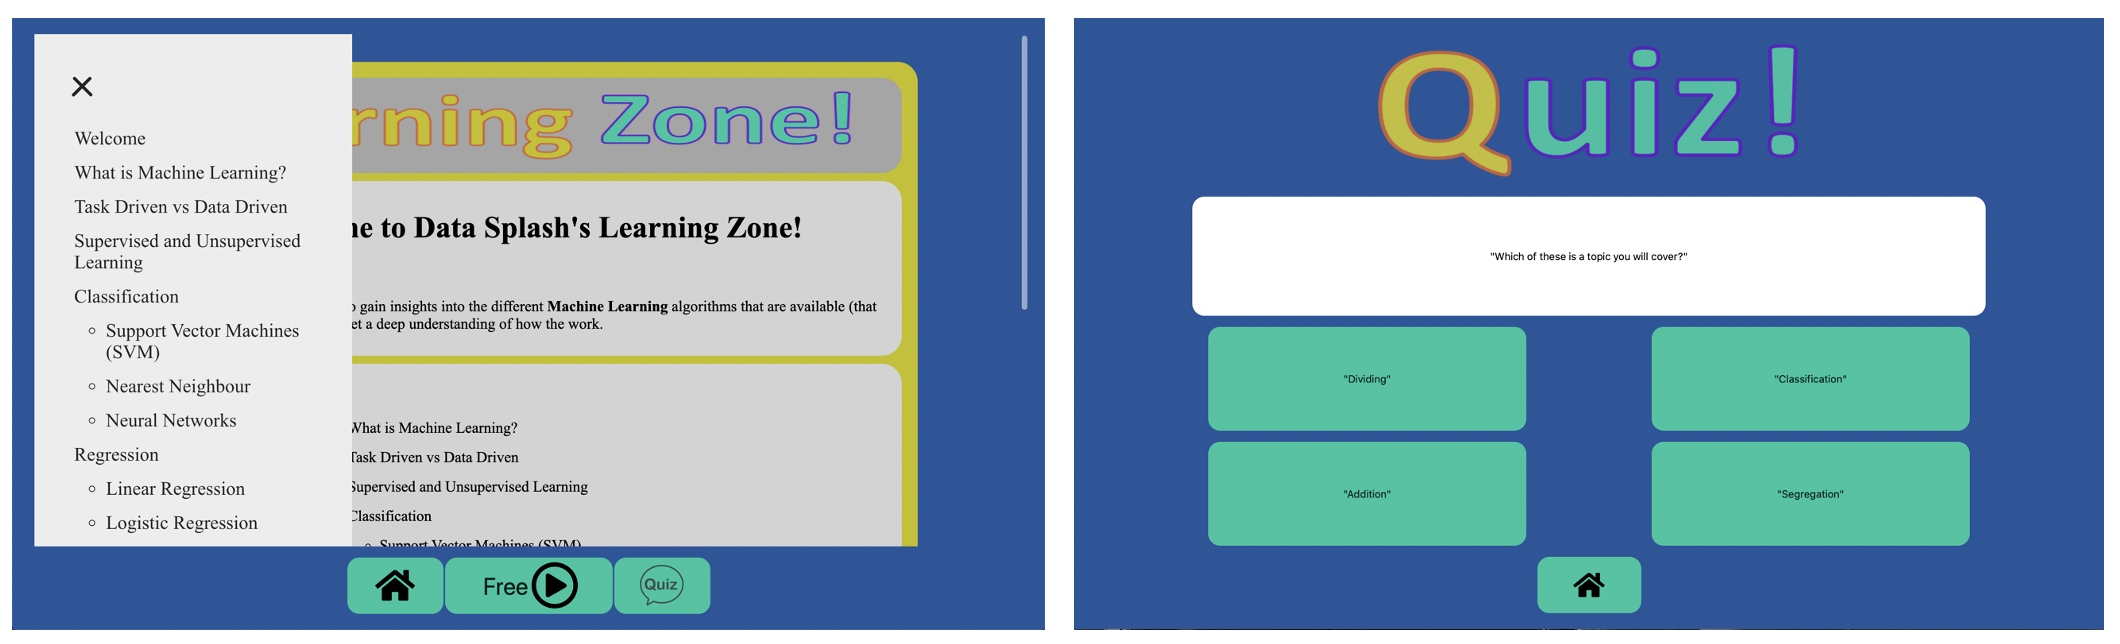
\includegraphics[width=15cm]{graphics/lz_navi_quiz.png}
				\caption{Demonstration of the navigation menu and the quiz section.}
				\label{fig:lz_navi_quiz}
			\end{center}
		\end{figure}
	
		The web pages follow a similar layout design. A blue background, a yellow background layer on top with an offset grey colour behind the text. Each page contains title at the top with a dark grey background. The content of the web pages either we an overview, for example, "Clustering", which looked into clustering as a whole and what the different types were. Alternatively, a web page would explain a specific algorithm, for example, "K-Means", which explained the intricacies of how the algorithm worked and the critical mechanics behind it.
	
		The three buttons at the bottom of the application screen trigger three different actions. All of which match to the intended buttons, a home button, to go back to the main menu, a free play button to send the player to the free play area with the intended algorithm that the user was learning about, and a quiz button which loads a multi-choice quiz.
	
	\begin{figure}[t]
		\begin{center}
			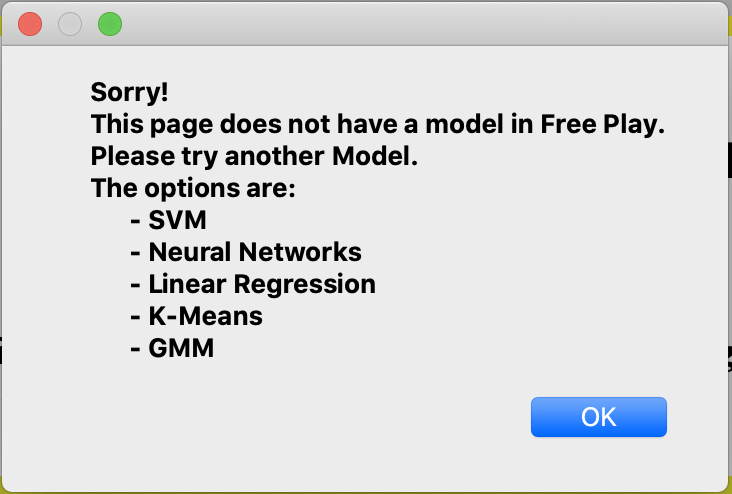
\includegraphics[width=6cm]{graphics/no_model_warning.png}
			\caption{An image displaying the warning message displayed to users.}
			\label{fig:no_model_warning}
		\end{center}
	\end{figure}
	
		When the player clicks the free play button, the application checks the HTML documents title tag and loads up the required model in the free play section. However, if the player clicks the button and the web page does not have a model available, within the free play section or it is just a general overview page, a message box will appear. The message box intension is to let the user know that they can not progress to the free play zone and a list of the available models (see fig: \ref{fig:no_model_warning}).
	
		The Quiz area is an additional area to the learning zone. The Quiz area is where the user can get tested on what they learned in the LZ area, in the form of a multiple-choice quiz. When the user is viewing a topic on the LZ, and they decide to take a quiz, the user will click on the quiz button, and this will read the title tags of the HTML document and open the required quiz. The quiz questions and answers are within their text file, and the name of the file matches the title tag's content. The text file itself holds the information in the format of a 2D array, that has the question at position zero, the answer at position one and then position 2 to 5 are the multiple-choice options. This information from the text file populates a question label and four buttons, allowing the user to click what button they think is the answer. The total of correct answers get added up and displayed to the user at the end in a message box.
	
	\subsection{Free Play Area}
	
		The Free Play (FP) zone is an area where the user gets to interact and play with different ML models. The models include Linear Regression, K-Means, Neural Networks, Linear Discriminant Analysis, Gaussian Mixture Models and SVM. The intension for the FP zone was to have all the models explained in the learning zone be available for the player to interact with, so it could help them fully understand how the model works by allowing the user to manipulate parameters and data points. However, due to time restrictions, there are only six models available, with 5 of the models having real interactivity but to different degrees.
		
		When the FP zone is accessed, unless accessed through the Learning Zone, a randomly selected model gets displayed to the user from the list mentioned before. On first glance, the user has multiple areas to either interact with or present information to them. The screen has a Widget that is linked to a Matplotlib library to handle PyQT5 backend interactions. Also, a model overview is displayed next to the widget, it tells the user information about the model, for example, the type of learning it is, supervised or unsupervised, the name of the model and a brief overview of the model. Just beneath the widget and overview is a group box that contains all the settings for the model and data interaction. The model settings group box contains combo boxes, radio buttons, checkboxes,  line edits and buttons, which all do different things depending on the model and data sets selected. Within the model settings group box, there are three additional group boxes. These are 'Model Attribute(s), 'Model Parameter(s)' and 'Data Options' with each group box displaying different content depending upon the model and data options selected in the combo boxes.
		
		\begin{figure}[t]
			\begin{center}
				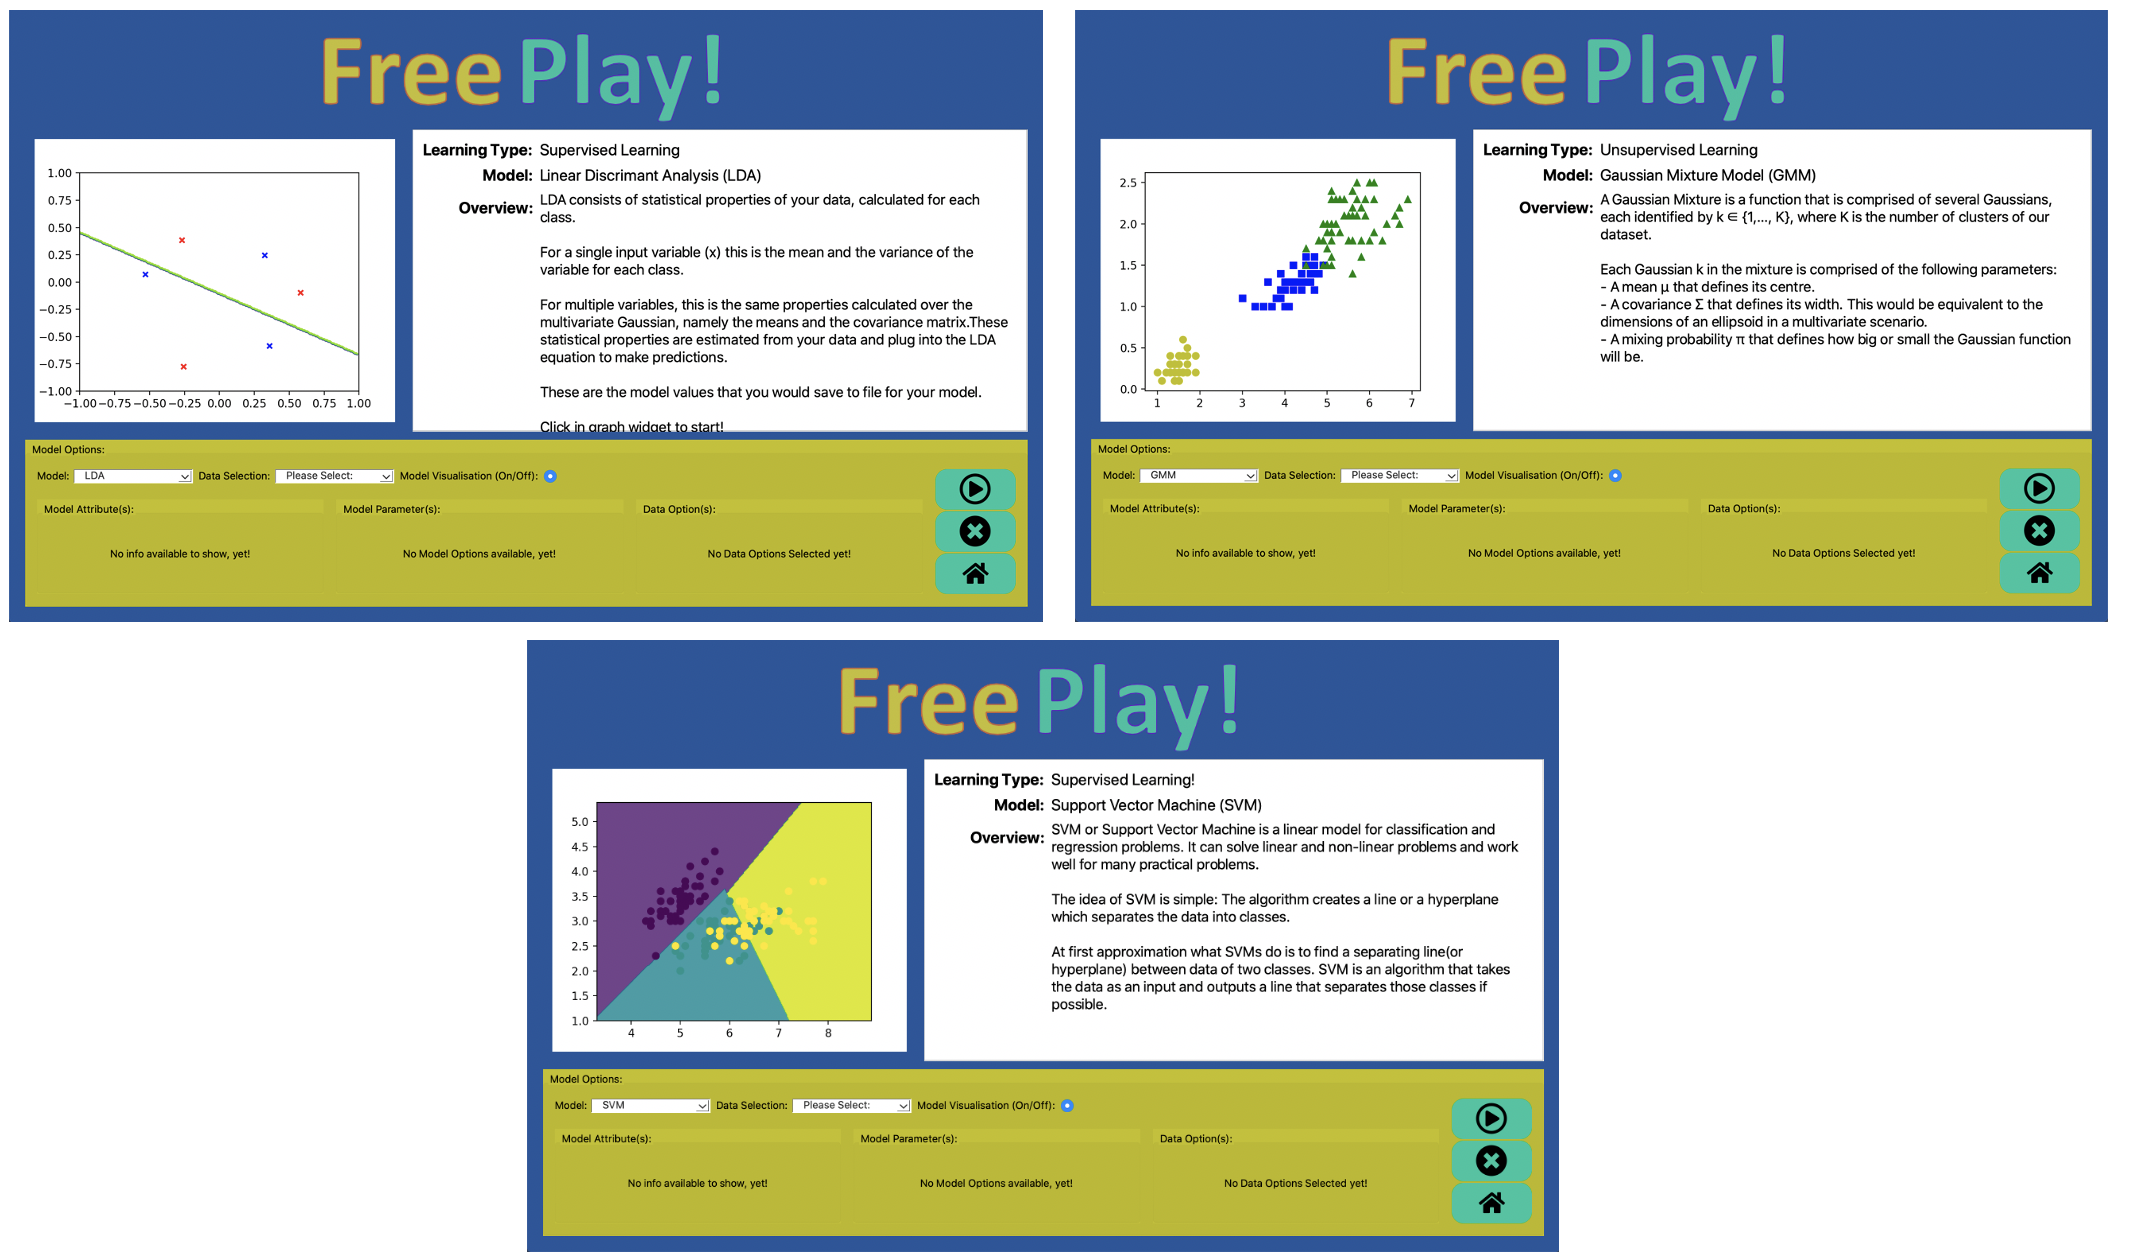
\includegraphics[width=15cm]{graphics/remaining_fp_examples.png}
				\caption{SVM, LDA and GMM UI screens.}
				\label{fig:others_example}
			\end{center}
		\end{figure}
		
		The model combo box contains six values, and these are 'Please Select', 'K-Means', 'LDA', 'Linear Regression', 'GMM', 'SVM', 'Neural Networks'. Once one of these options is selected, apart from the 'Please Select', the desired model will display in the Matplotlib widget area. The Model attributes and parameters boxes will display the required information unless the models 'LDA', 'SVM' and 'GMM' are selected (see fig: \ref{fig:others_example}). Instead, a label placeholder saying, 'No Options available, yet!' will be displayed. While LDA has a fully interactive model in the MatplotLib widget, it does not present options for the user to change within the model, the user can only click on the widget and place points, which the model will then apply and create the required actions. Therefore a place holder label appears stating to click in the game widget to interact with the model. While LDA and GMM both have the ability for the model visualisations to toggle on and off, showing how the models have fit their data, GMM has little much additional functionality. GMM only allows the user to toggle on and off the visualisation, which is the model predicting the 'Iris' dataset clusters. However, SVM only displays the model's output, again using the 'Iris' data set, but the output shows the boundary lines and area that each partition covers.
		
		While on the other hand, the Linear Regression, K-Means and Neural Network models display different options. Linear Regression displays to the user labels in the attributes group box to show them the values for the intercept, estimated coefficient and outcome. There is also a line edit available for the user to input a value and see what the model would predict out, which gets displayed in the output label. However, Linear Regression does not have any model parameters, and this is due to the values getting deemed as not having much impact on the model and limited implementational time. 
		
		\begin{figure}[t]
			\begin{center}
				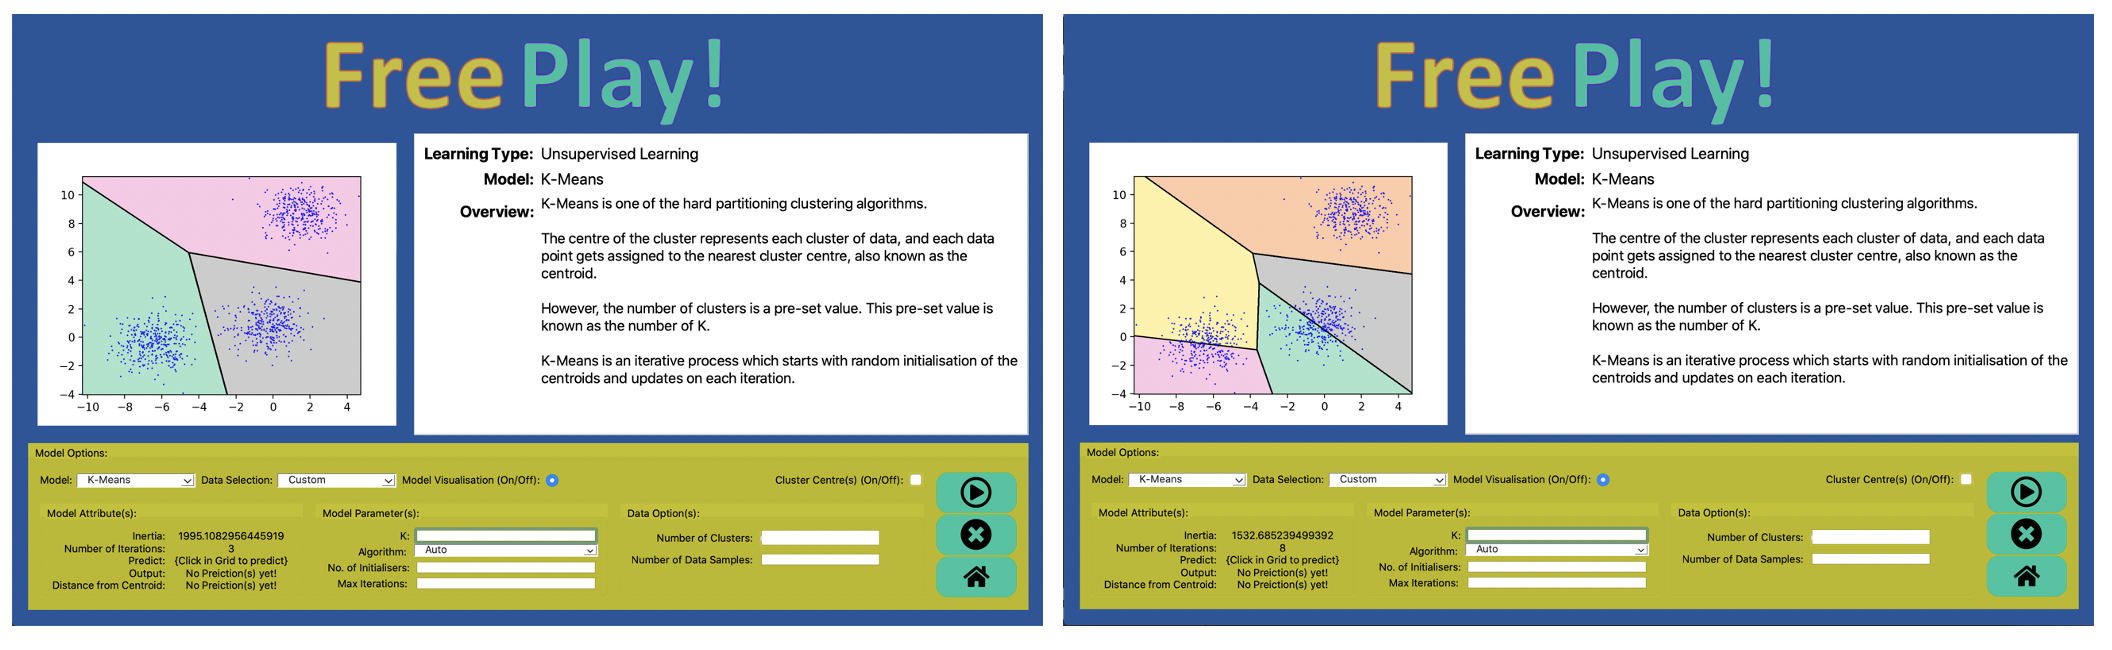
\includegraphics[width=15cm]{graphics/chaning_k_fp_example.png}
				\caption{A comparison of the K-Means k value unchanged ($k=3$) when creating the dataset and then being changed by the user ($k=5$).}
				\label{fig:km_example}
			\end{center}
		\end{figure}
		
		When K-Means gets selected (see fig: \ref{fig:km_example}), both the attributes and parameters group boxes have information and selection options displayed to the user. The attributes group box displays the information for Inertia, the number of iterations that got performed fitting the data, prediction, which relies on the user to click within the Matplotlib widget and the X and y coordinates get displayed along with a cluster prediction label in the output label. There is also a distance from the centroid value displayed, and this value got achieved by using the SKLearn Metrics library. The model parameters group box displays multiple line edits and a combo box that allows the user to input values to the model. These will alter the K-Means k value (number of clusters), the number of initialisers, the max number of iterations and the underlying algorithm (auto, full or Elkan), that gets used.  The k value is independent of the number of clusters in the data options, so they do not impact on each other. Allowing the k value to be changed independently will allow the user to be able to experiment with the model to see how two, three or other k values affect the prediction, even when known that the data may have, for example, five different clusters. K-Means also brings up an additional option, and this is to be able to switch on and off the centres of the clusters. When the checkbox gets enabled, this will lay on top of the data points an 'X' where each of the cluster centres is and when it is disabled, it will remove the 'X'.
		
	
		[NN Att no. of layers/ neurons -> params set the values. Not implemented in-app yet!]
		
		\begin{figure}[t]
			\begin{center}
				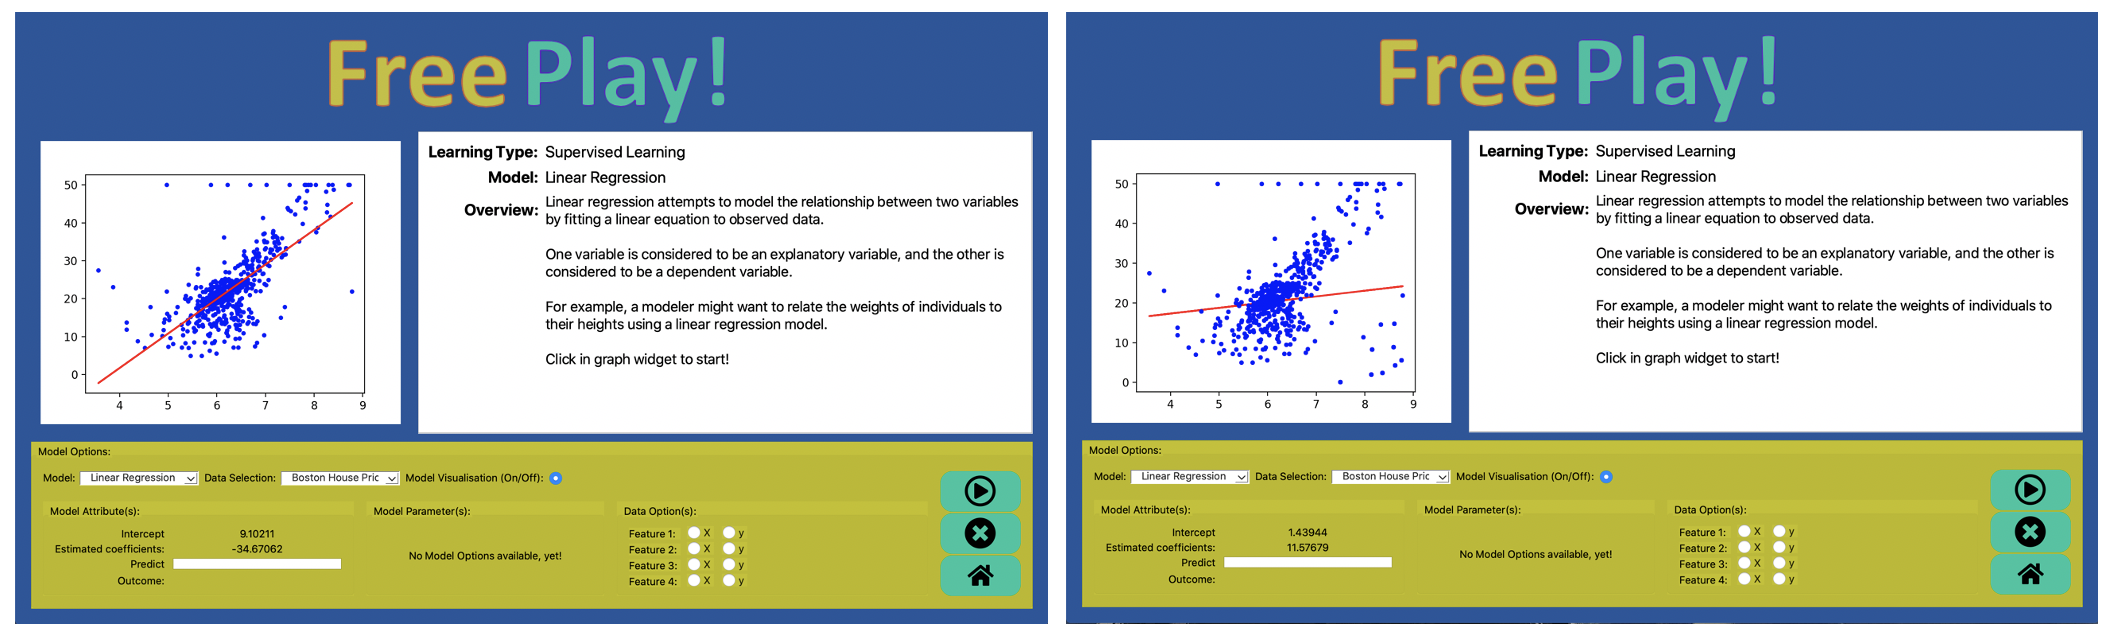
\includegraphics[width=15cm]{graphics/manipulating_lr_data.png}
				\caption{Extra data points have been added by clicking with the plot widget and therefore changing the models prediction fit.}
				\label{fig:manipulating_lr_data}
			\end{center}
		\end{figure}
	
		\begin{figure}[t]
			\begin{center}
				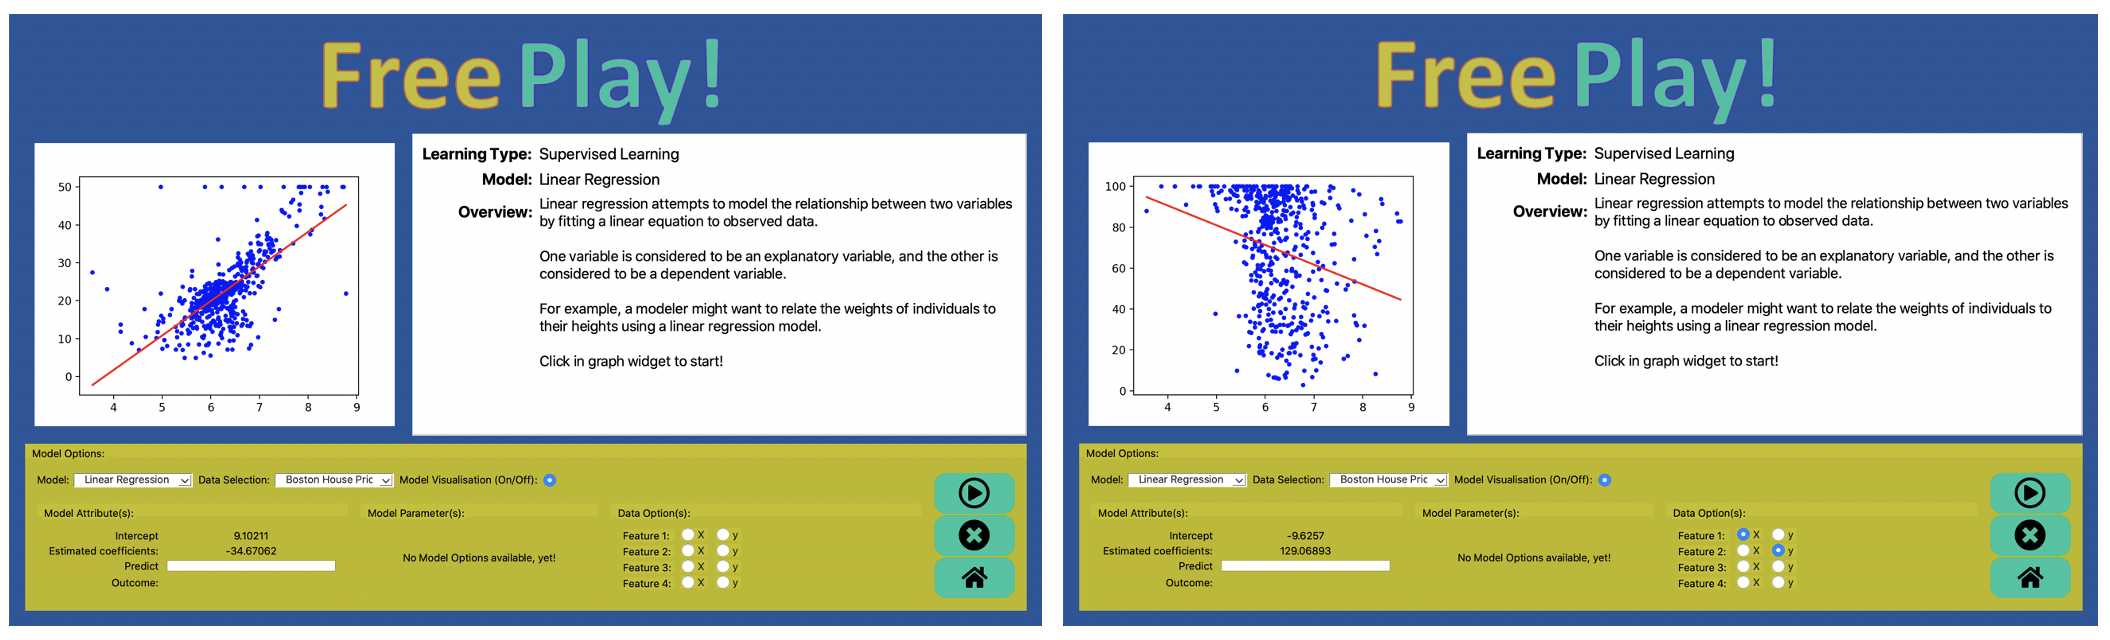
\includegraphics[width=15cm]{graphics/lr_changing_xy.png}
				\caption{The player changing the features selected for the linear regression model.}
				\label{fig:lr_changing_xy}
			\end{center}
		\end{figure}

		\begin{figure}[t]
			\begin{center}
				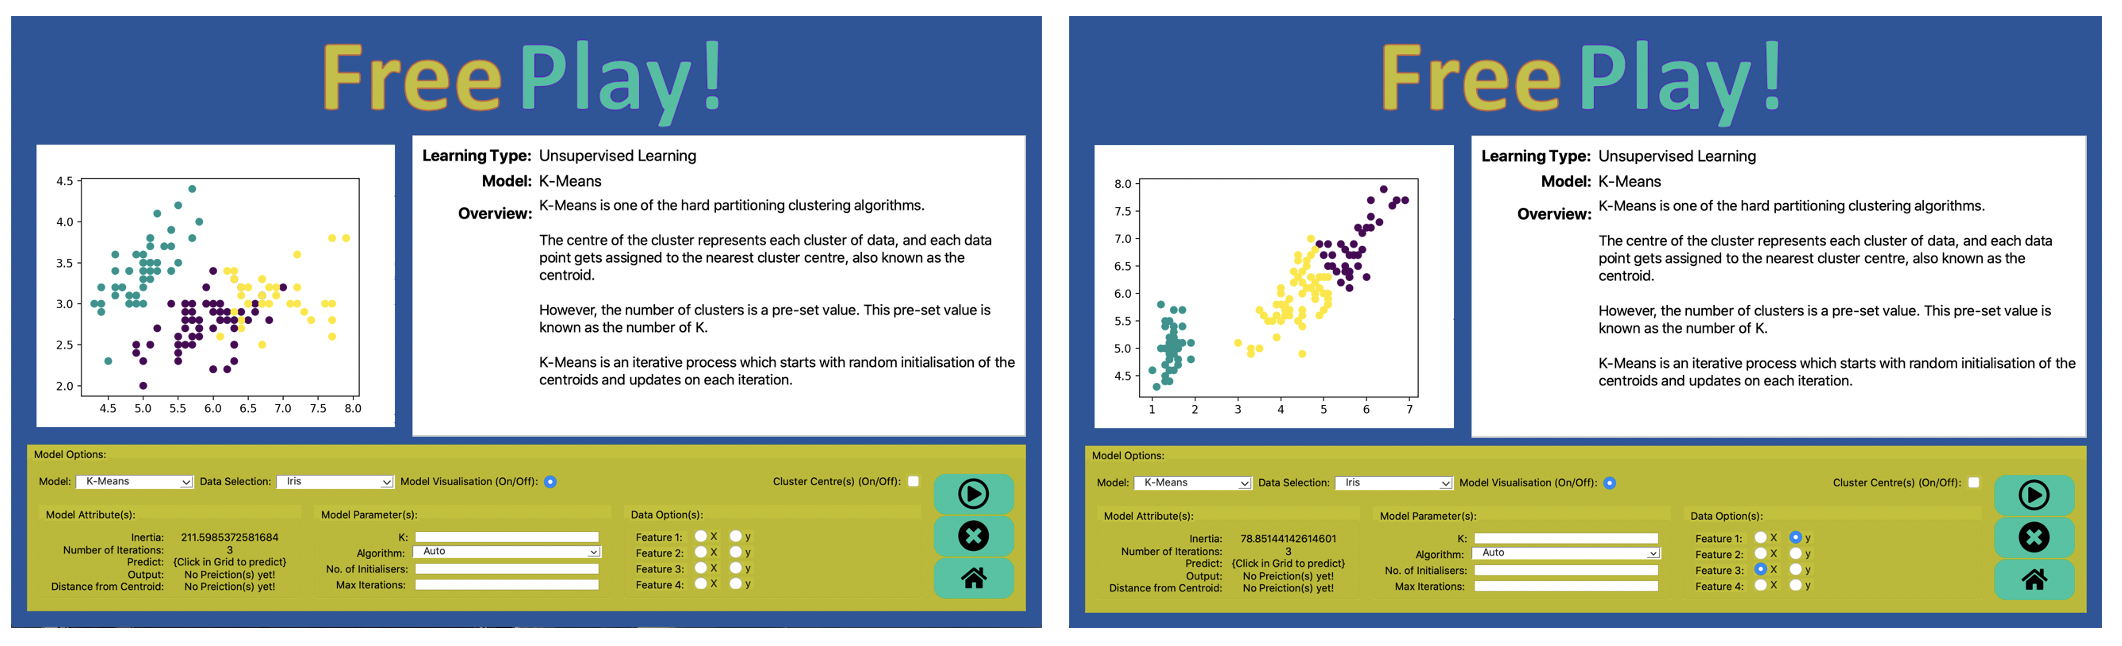
\includegraphics[width=15cm]{graphics/km_change_xy.png}
				\caption{The player changing the features selected for the k-means model.}
				\label{fig:km_change_xy}
			\end{center}
		\end{figure}
		
	
		The data combo box displays the data options for the different models and depending on what option is selected depends on the information that is on offer to the user in the data options group box. If the custom data option is selected, then the group box will display different options to the user to be able to generate custom data points to be displayed in the Matplotlib widget game screen. The only models that have this option are the Linear Regression and K-Means models. Linear Regression has the data options 'Diabetes' and 'Boston House Prices' and K-Means has the data options 'Iris' and 'Moons'. When these are selected, the data option displays radio button options for the user to select the features they would like the model to display, on the X and y-axis, and get fitted. Linear Regression's 'Custom' data option allows the user the ability to change the random generated data's settings. These settings include the number of data samples and if there are any outliers wanted, if so then an option to add the number of outliers. Whereas K-Means 'Custom' data option allows the user the ability to change the number of clusters to generate and the number of data samples wanted. The other models have a label placeholder saying, 'no data options selected yet!' and no actual data selection options. In the case of LDA and Neural Network, this is more due to the decision we made. Based on the way the model's fit function was implemented, not allowing the user to generate random data was decided. Doing so would impact on how the model gets interacted with by the user. However, in the case of the other models, it was a lack of time that impacted the inability to add this feature. Though, it was always the intention to add it.
		
		The final aspects of the Model options group box are three buttons, a play button, a clear button and a home button. Where the home button is self-explanatory in terms of returning the user to the main menu, and the clear button resetting the Matplotlib Widget axis contents. The play button is where the primary handling of how the user interacts with the back end of the models and datasets. When the user inputs information, they are required to press the play button for these features to be implemented.
	
	
	
	\subsection{Achievements Area}
	The intensions for the Achievement Area was displaying to the user all of the gamification badges available. Providing an overview and hits on how to unlock them. The achievements were going to have a bronze, silver and gold level, and we planned to be unlocked once the user had completed specific tasks like playing the game three times or completing a quiz. However, due to time limitation, this was not possible, and the application, as it currently stands, displays a coming soon image and button for the user to navigate back to the main menu.
	
	
	\section{Example user stories (A UML term for case studies or example playthroughs)}
	\label{sec:ide_used}
	
	
	

	\chapter{Conclusions and Future Work}
\label{chap:conclusion}

In this document we have demonstrated the use of a LaTeX thesis template which can produce a professional looking academic document. 

\section{Contributions} 
\label{sec:conclusion_contributions}

The main contributions of this work can be summarized as follows:
\begin{description}	

	\item[$\bullet$ A LaTeX thesis template]\hfill
	
	Modify this document by adding additional top level content chapters. These descriptions should take a more retrospective tone as you include summary of performance or viability. 
	
	
	\item[$\bullet$ A typesetting guide of useful primitive elements]\hfill
	
	Use the building blocks within this template to typeset each part of your document. Aim to use simple and reusable elements to keep your document neat and consistently styled throughout.
	
	\item[$\bullet$ A review of how to find and cite external resources]\hfill
		
	We review techniques and resources for finding and properly citing resources from the prior academic literature and from online resources. 
	
\end{description}

\section{Future Work}
\label{sec:conclusion_future_work}

Future editions of this template may include additional references to Futurama.
	
% Formatting citations properly when they are rendering incorrectly in your PDF can be fiddly,
% espectially when punctuation and international characters are involed. Sometimes multiple re-compilations
% are needed in addition to clearing temporary auxiliary files to see your changes in your document.
% Insert the bibliography using citations contained in the file citations.bib
	\bibintoc%
	\bibliography{citations} 
	
% In the appendix you might include a full code listing for an implemented algorithm that you showed a 
% small chunk of in one of your chapters. If you have extra graphs for ablation style experiments you 
% might enumerate them within the appendix and use \label{name} and \ref{name} to automatically insert 
% the correct section locations when you talk about them in your chapters.
% Within appendix.tex you should use chapters as the top level section dividers.
	\appendix
	\addappheadtotoc
	\chapter{User Study Questionnaire}
\label{app:user_study_q}

% Code listings should live in a code file, not embedded directly into your LaTeX code!
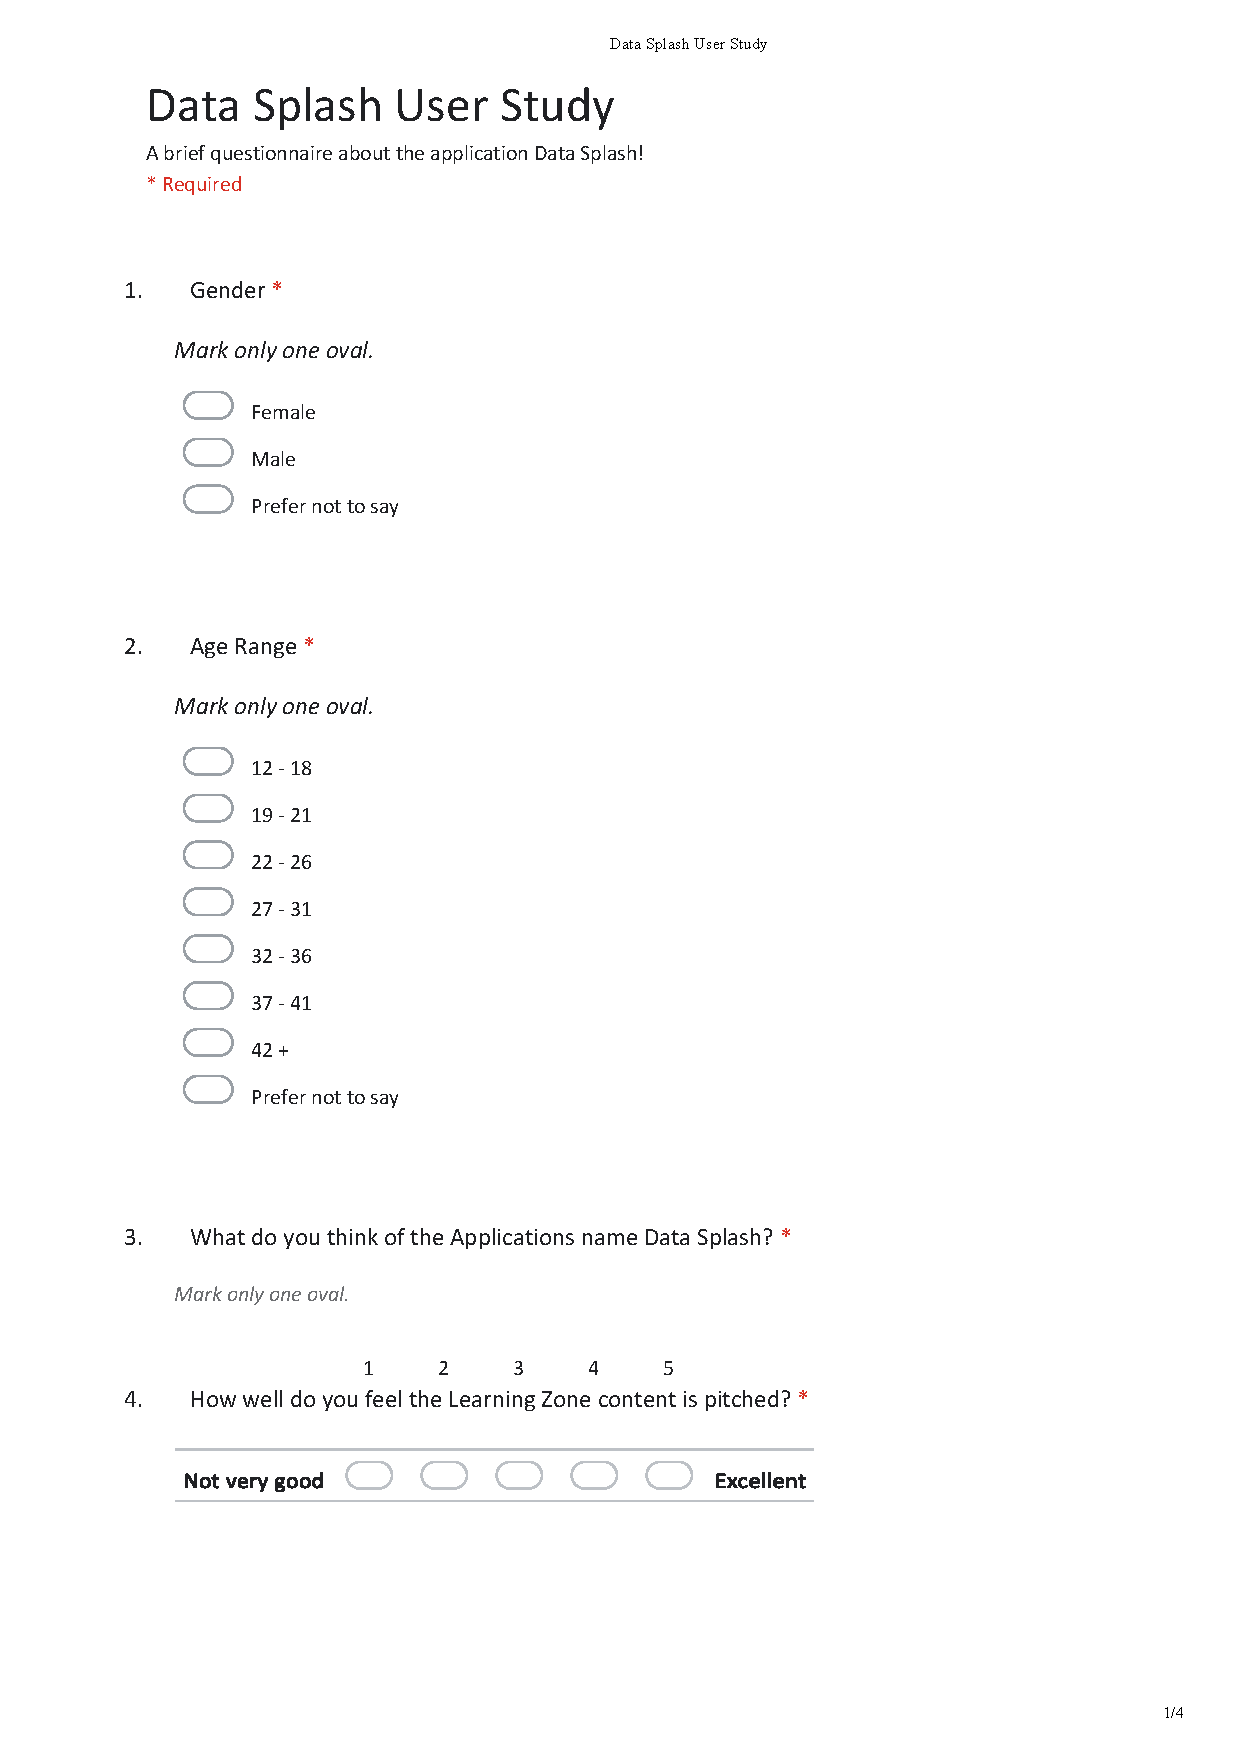
\includepdf[pages=1-4]{DS_User_Study.pdf}
\label{app:supplementary_data}

%\lstinputlisting[language=python, label={lst:python_nn}, caption={The Neural Network Gamboard Class}]{./listings/nngameboard.py}


	
\end{document}